%%%%%%%%%%%%%%%%%%%%%%%%%%%%%%%%%%%%%%%%%%%%%%%%%%%%%%%%%%%%%%%%%
% Qualificacao de Doutorado / Dept Fisica, CFM, UFSC            %
% Eduardo@UFSC - 2015                                           %
%%%%%%%%%%%%%%%%%%%%%%%%%%%%%%%%%%%%%%%%%%%%%%%%%%%%%%%%%%%%%%%%%

%:::::::::::::::::::::::::::::::::::::::::::::::::::::::::::::::%
%                                                               %
%                          Capítulo 3                           %
%                                                               %
%:::::::::::::::::::::::::::::::::::::::::::::::::::::::::::::::%

%***************************************************************%
%                                                               %
%                     Comparação SFR EML                        %
%                                                               %
%***************************************************************%

\chapter{Propriedades da síntese e propriedades nebulares}
\label{sec:synvsneb}

\section{Amostra de galáxias}
\label{sec:synvsneb:amostra}

Neste trabalho estamos interessados em estudar a formação estelar recente em discos de galáxias.
Nossa amostra começa conténdo todas as 226176 regiões (zonas) das 305 galáxias espirais do CALIFA
{\em Survey}. Cada uma dessas zonas dessa é composta por um ou mais píxels, com um espectro
resultante da soma dos espectros destes, para que tenhamos relação sinal-ruído maior ou igual a 20
na janela de normalização do espectro resultante. Esse procedimento, conhecido como {\em Voronoi
binning}, está detalhado, juntamente com o procedimento de derivação das propriedades estelares
através do código \starlight para cada uma das regiões destas galáxias, em
\citet{CidFernandes.etal.2013a}.

\subsection{Classificação Morfológica}
\label{sec:synvsneb:amostra:morf}

Com tipos morfológicos variando entre Sa e Sd, massas estelares entre $10^9$ e $10^{11.5}\ M_\odot$
e populações estelares com idades médias entre $10^8$ e $10^{10}$ anos, podemos ver na Fig.
\ref{fig:amostraMorf} que as galáxias se ordenam de forma interessante quando agrupadas por tipo
morfológico, anticorrelacionando com a idade média estelar e a massa estelar ($M_\star$ e $t_\star$)
e correlacionando com a fração de luz proveniente das população jovens ($x_Y \equiv x_Y(t_\star <
t_{SF})$). Cada galáxia contribui com um ponto em cada painel deste gráfico, ou seja, são
propriedades integradas. Os intervalos entre primeiro e terceiro quartil quase não se sobrepõem no
quando analisamos as classes morfológicas por idade média. O resultado parece ser muito interessante
visto que a classificação morfológica foi feita por colaboradores do CALIFA totalmente através de
inspeção visual das imagens na banda-r do \SDSS das mesmas galáxias. Vemos também que as galáxias
tipo Sd possuem as populações estelares mais jovens e menos massivas na média. Por ser um fenômeno
apenas de posição do referencial de observação não deveríamos ver preferência por valor de relação
de semi-exios (b/a) quando dividimos em classes morfológicas, o que realmente acontece.

\begin{figure}
	\centering
	%\resizebox{0.99\textwidth}{!}{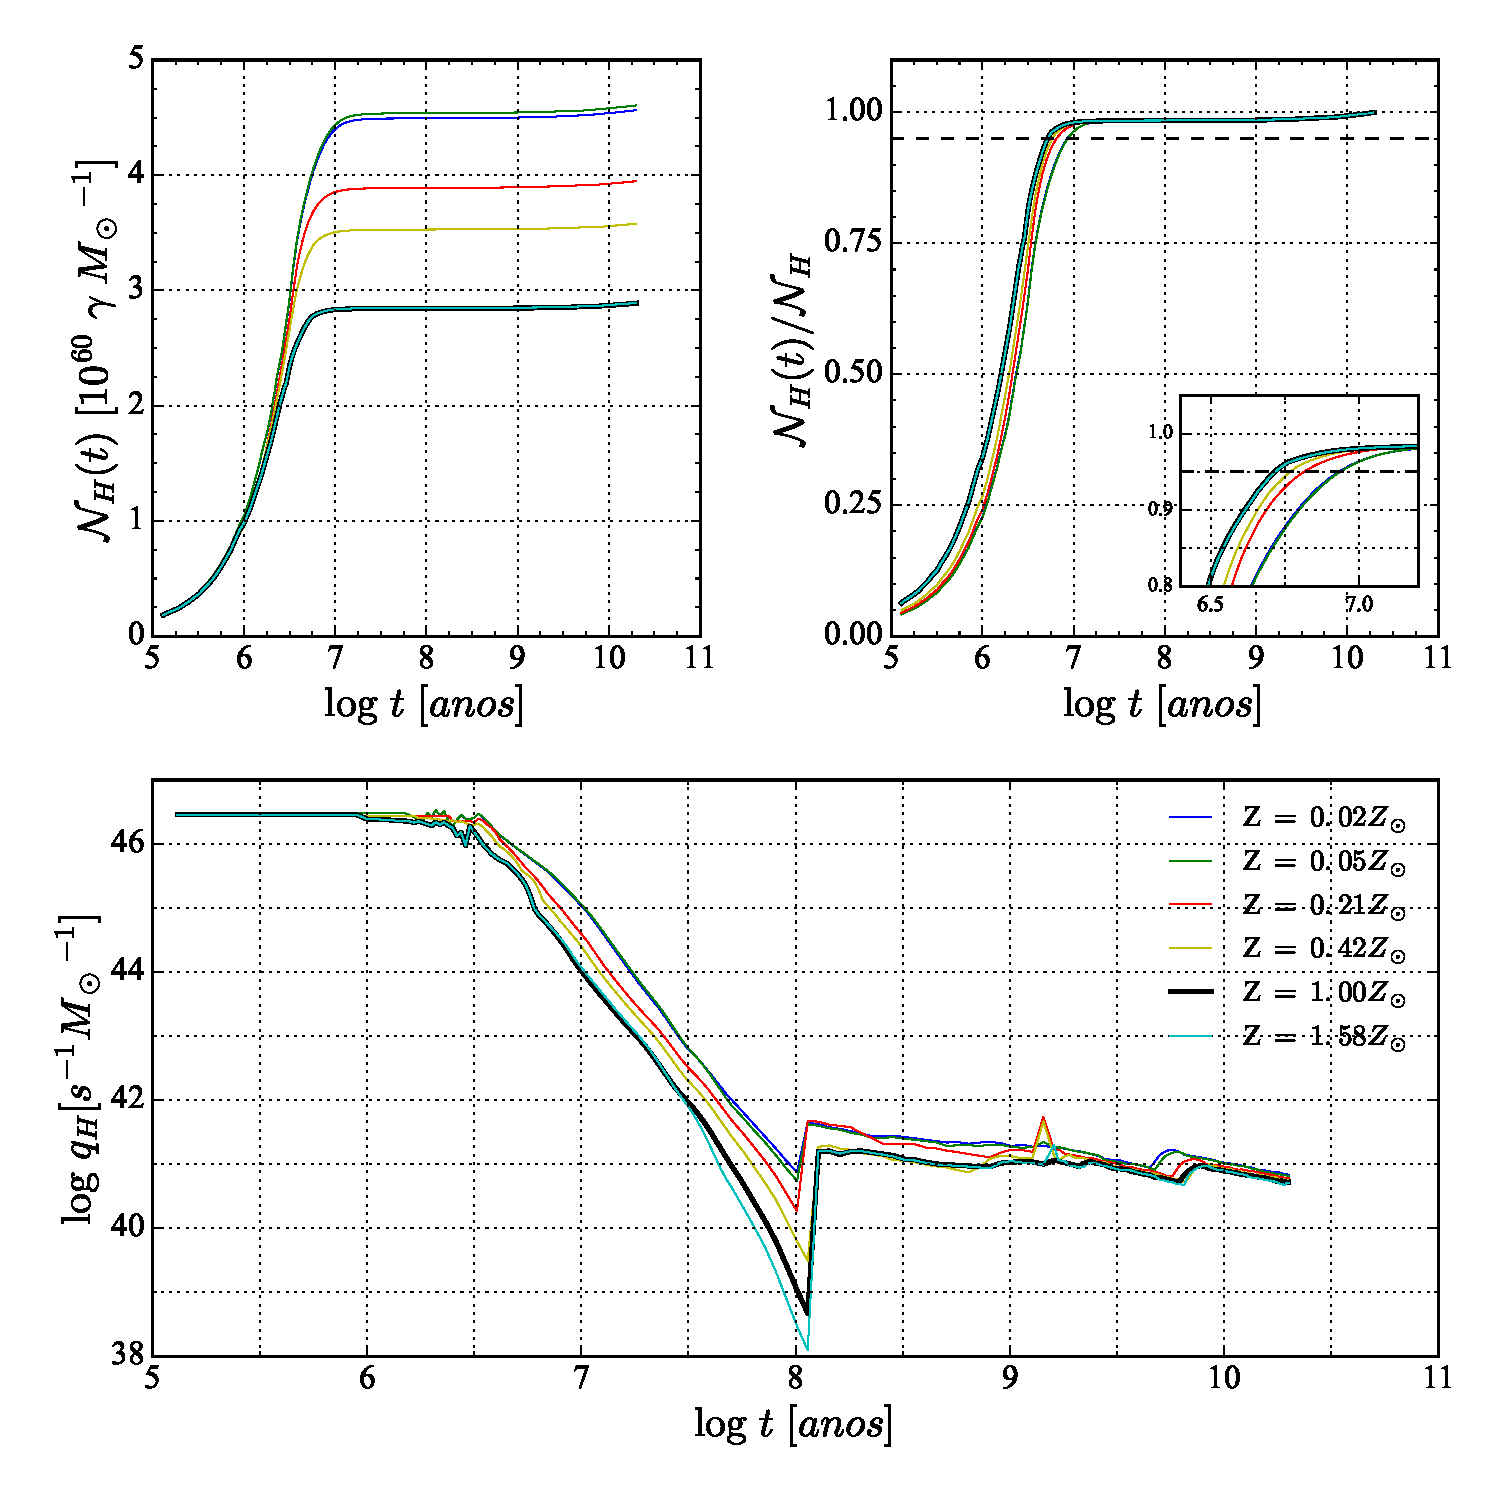
\includegraphics{Nh_logt_metBase_Padova2000_salp.pdf}}
	\resizebox{0.99\textwidth}{!}{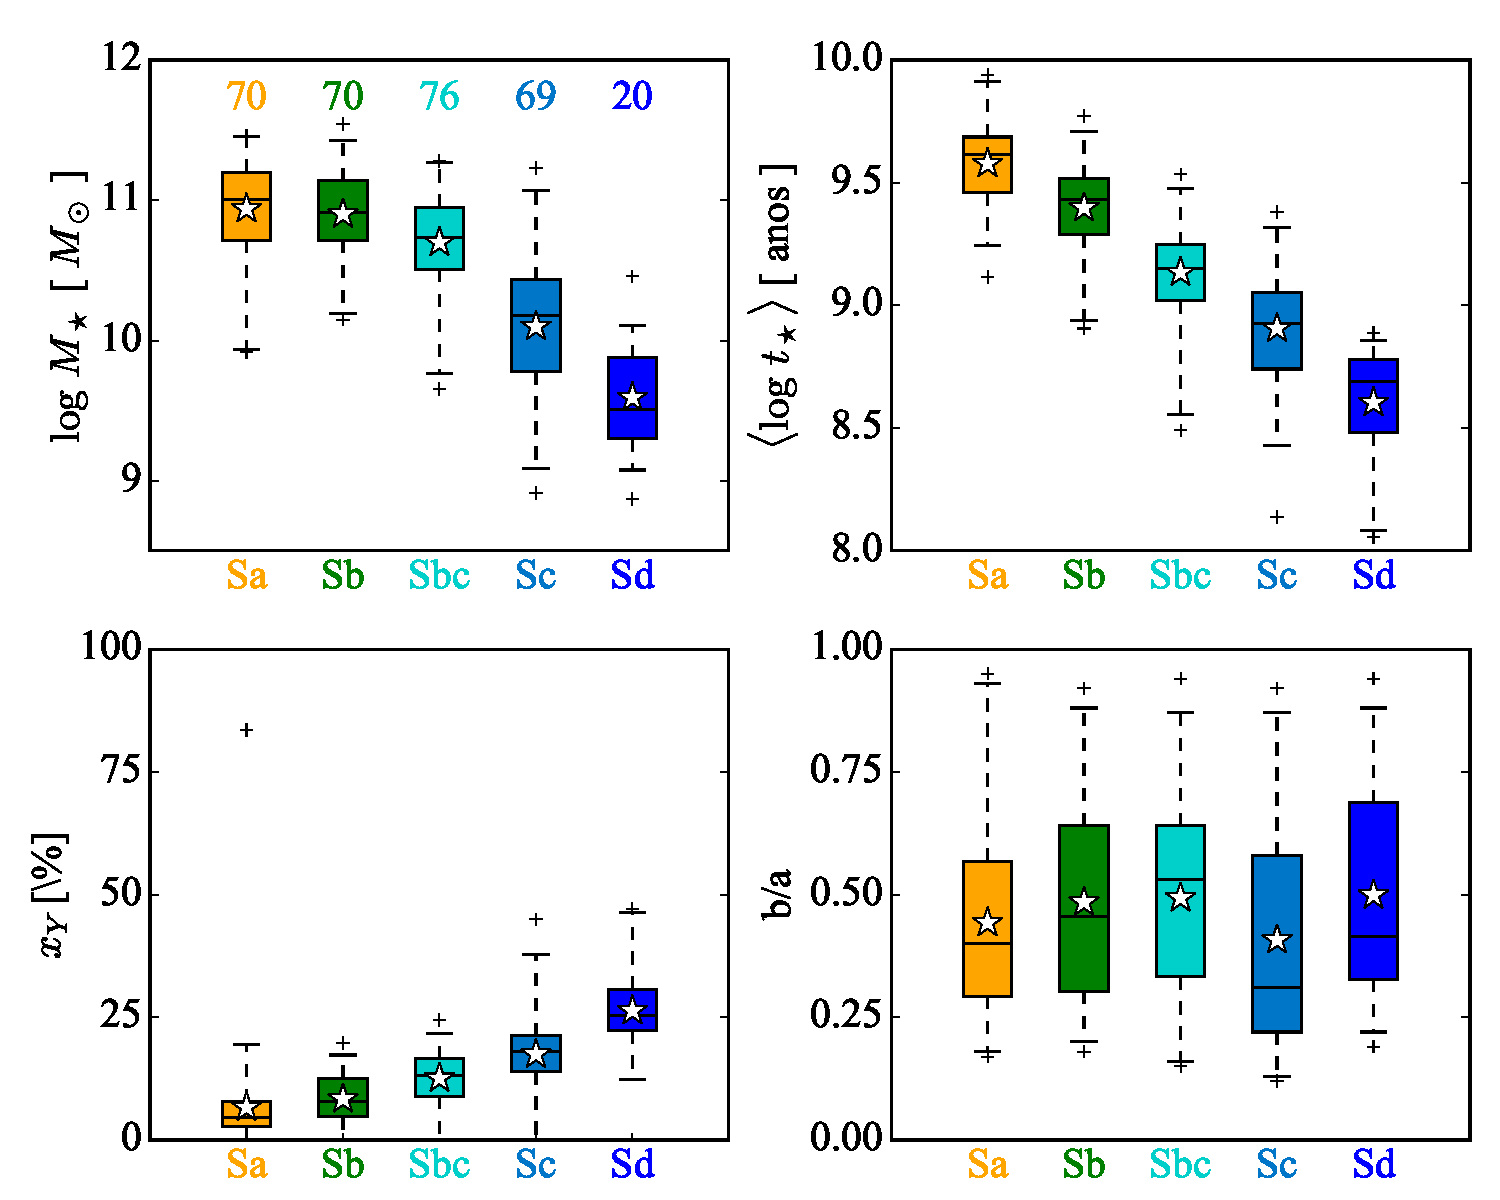
\includegraphics{figuras/sample_morf.pdf}}
	\caption[Classificação por morfologia.]
	{\emph{Em sentido horário a partir do painel superior esquerdo}: gráfico da massa estelar, idade
	estelar média, fração de luz proveniente das população jovens ($x_Y \equiv x_Y(t_\star < t_{SF})$) e
	inclinação, divididos em classes morfológicas para 305 galáxias espirais da amostra total do
	CALIFA. No primeiro painel, temos o número de galáxias dentro de cada classe morfológica. Cada
	caixa tem altura definida pelo primeiro e terceiro quartil da distribuição dentro de um tipo
	morfológico. Uma faixa preta marca a mediana e uma estrela a média. Em cada caixa, a linha
	pontilhada vertical se estende mostrando o intervalo de $3\sigma$. Valores que ficam fora do
	intervalo de $3\sigma$ são marcados por uma cruz vermelha.}
	\label{fig:amostraMorf}
\end{figure}

Estamos em fase de finalização de um artigo aonde comparamos a relação entre a taxa de formação
estelar e a massa para diferentes classes morfológicas. Esse artigo deve sair por meados de 2016.

\subsection{Mascarando elementos e removendo {\em outliers}}
\label{sec:synvsneb:amostra:mask}

Para que possamos focar nossos estudos às regiões de formação estelar, aplicamos uma máscara nos
dados selecionando as regiões que possuam:
\begin{itemize}
  \item medidas do fluxo integrado das linhas de \Hbeta, \oIII, \Halpha e \nII com relação
sinal-ruído maior do que 3;
  \item medidas para as seis propriedades comparadas neste capítulo ($\tauVS$, $\tauVN$,
$\SigmaSFR$, $\SigmaSFRN$, $\meanM{\log Z_\star}$ e $\log(O/H)$);
  \item fração de população estelar jovem ($t_\star < t_{SF}$) maior que 5\% ($x_Y > 5$\%);
  \item $\tauV$ e $\tauVN$ maiores que 0.05;
  \item mais do que cinco zonas contribuindo para o cálculo dos perfis radiais (ver
  \ref{sec:synvsneb:amostra:rad});
  \item distância maior que 70\% do raio que contém metade da luz ({\em half-light radius} - HLR).
\end{itemize}
\noindent O que aqui chamamos de população jovem discutiremos um pouco mais adiante, na Sec.
\ref{sec:synvsneb:SFR}. última imposição é feita para que não haja contaminação por zonas
do bojo da galáxia (partes centrais onde as linhas são produzidas por diferentes fenômenos físicos,
relacionados a um núcleo ativo). Esse valor (0.7 HLR) foi definido por nossos colaboradores
analisando as curvas de brilho das galáxias e representa um valor máximo para localização de zonas
centrais. Ao final, produzimos a Fig. \ref{fig:amostraRealMorf} da mesma forma que a Fig.
\ref{fig:amostraMorf}, mas com a densidade superficial de massa ao invés da massa, pelo fato de que
as zonas não possuem mesma área. Nos sobram 16840 zonas de 199 galáxias (21 Sa, 42 Sb, 63 Sbc, 59 Sc
e 14 Sd). Podemos ver que as tendências observadas na Fig. \ref{fig:amostraMorf} não se alteram após
estes cortes.

\begin{figure}
	\centering
	%\resizebox{0.99\textwidth}{!}{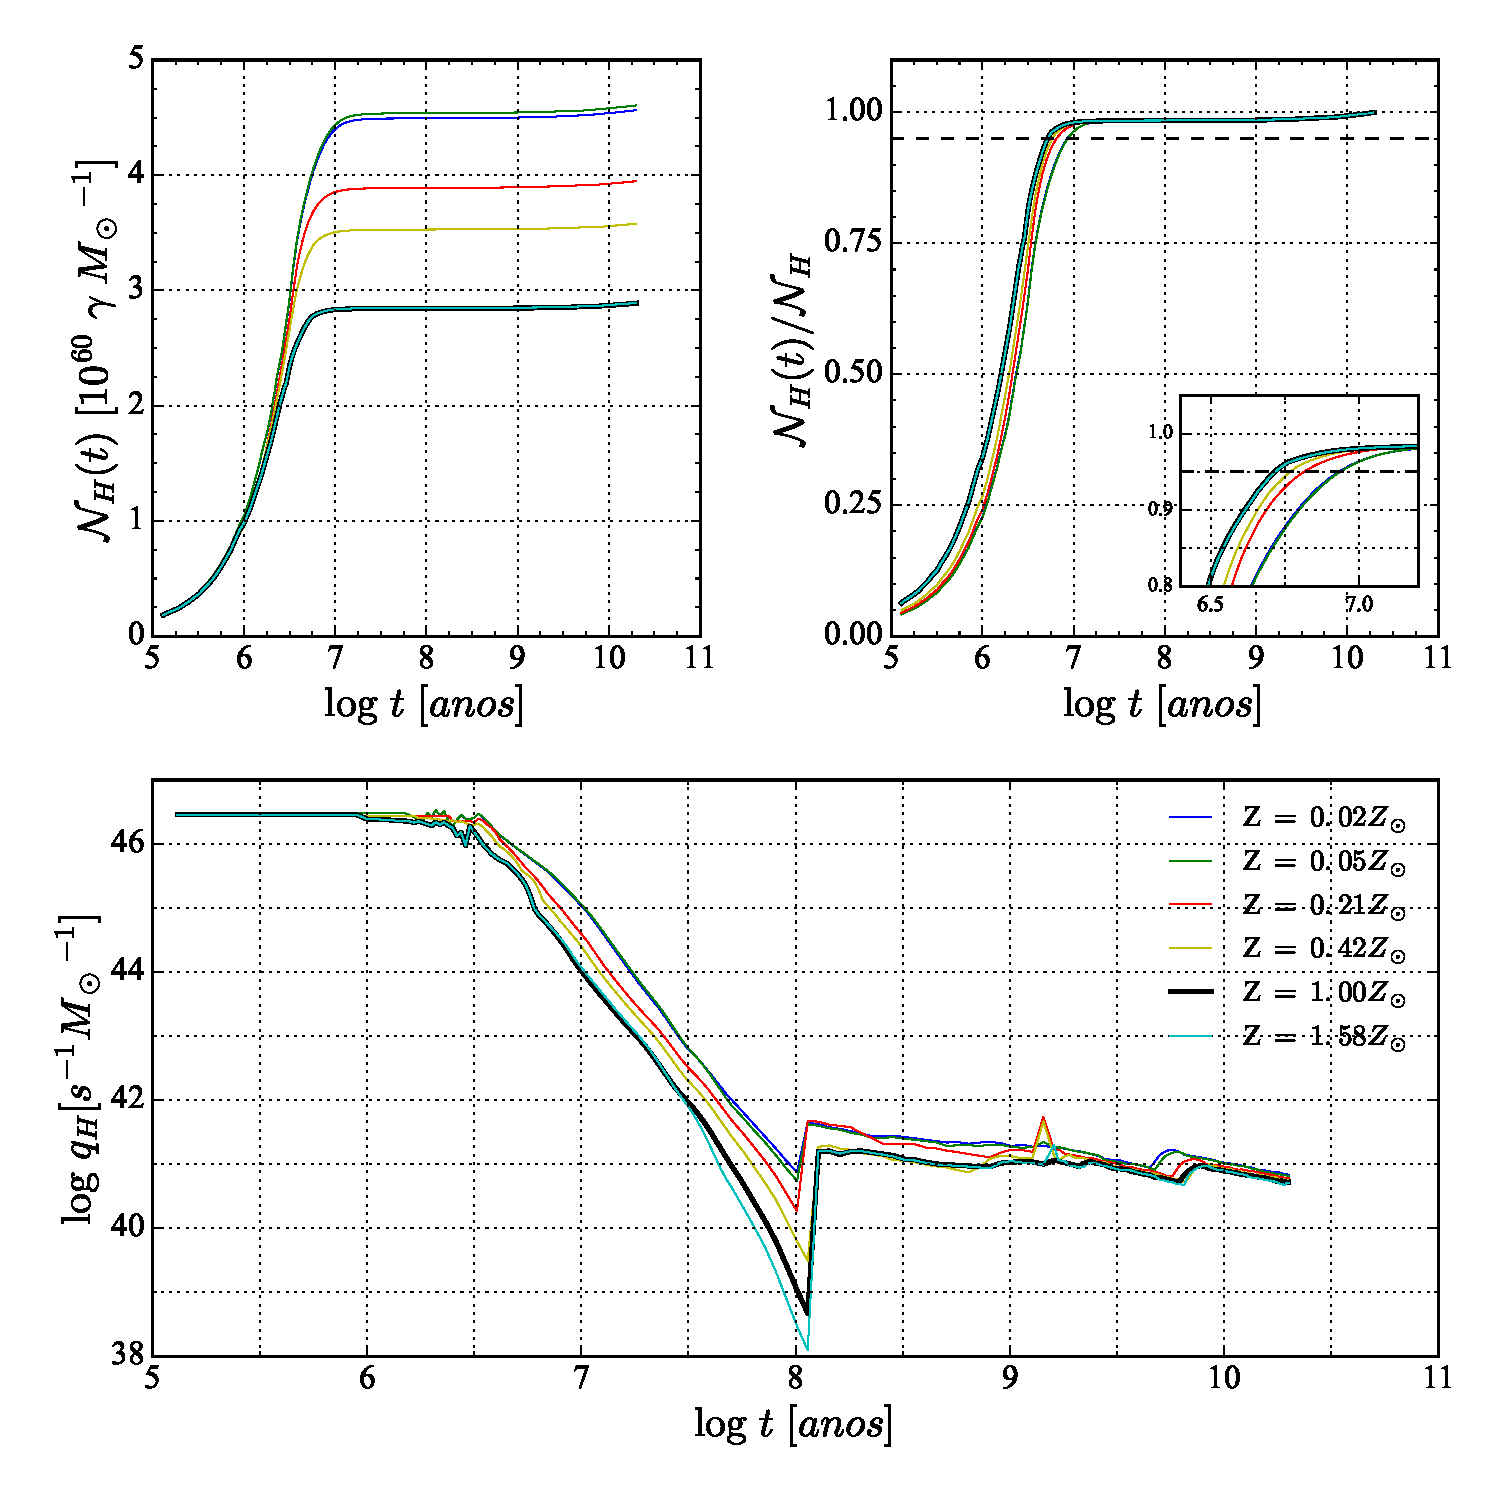
\includegraphics{Nh_logt_metBase_Padova2000_salp.pdf}}
	\resizebox{0.99\textwidth}{!}{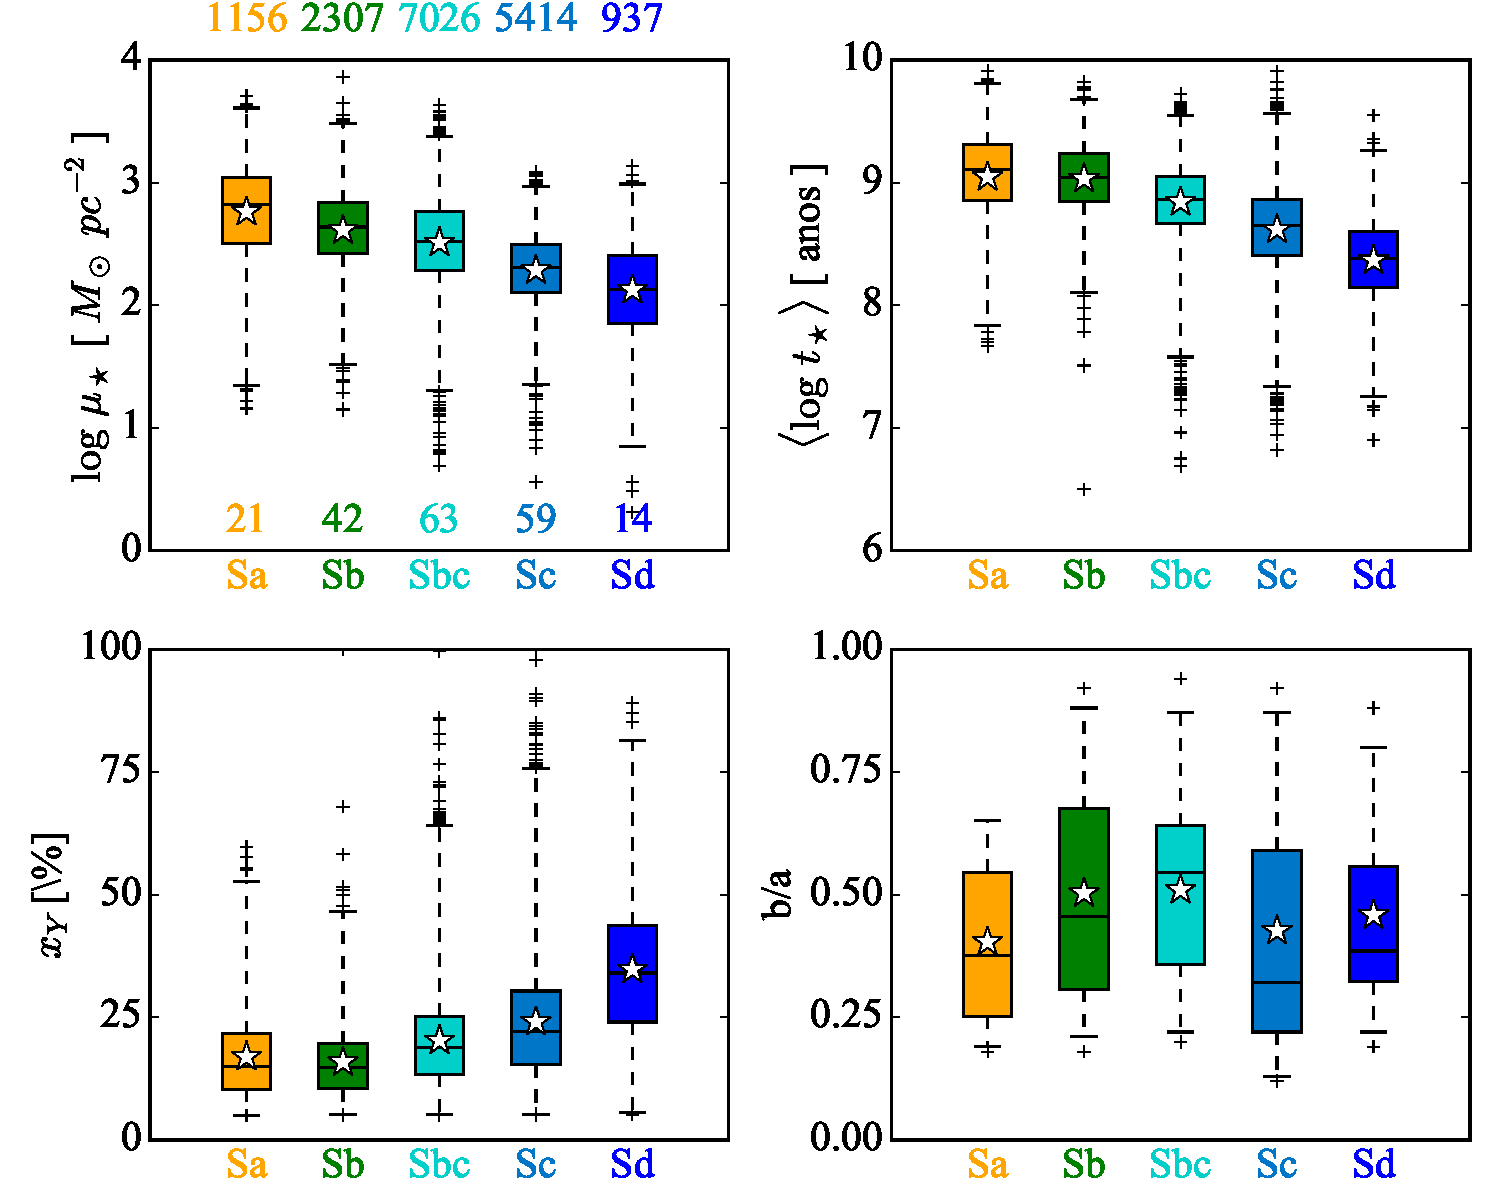
\includegraphics{figuras/sample_real_morf_zones.pdf}}
	\caption[Classificação por morfologia após máscara.]
	{Mesma ideia da Fig \ref{fig:amostraMorf} no entanto para todas as zonas restantes após a
	aplicação da máscara discutida em \ref{sec:synvsneb:amostra:mask}. No painel superior esquerdo
	temos a densidade superficial de massa, diferentemente da Fig. \ref{fig:amostraMorf} pois as zonas
	possuem números diferentes de píxeis, portanto, áreas diferentes. Também podemos ver acima deste
	painel o número de zonas contidas em cada classe morfológica. Vemos que as tendências notáveis para
	os valores integrados se mantém quando analisamos os resultados por zona.}
	\label{fig:amostraRealMorf}
\end{figure}

\subsection{Perfis radiais}
\label{sec:synvsneb:amostra:rad}

Uma maneira interessante de analisar galáxias é produzir perfis radiais para as propriedades
físicas. Esse tipo de média azimutal (tanto em classes definidas por anéis circulares quanto em
anéis elípticos) diminui o espalhamento dos pontos. Para a análise individual de cada galáxia também
permite estudo da evolução das propriedades ao longo do raio. Quando colocamos todas as galáxias na
mesma análise, a vantagem dos {\em bins} radiais vem do balanceamento da influência de cada galáxia
quando analisamos todas juntas. Para que seja possível este ``empilhamento'' de galáxias, estas
médias radiais são feitas definindo-se um raio efetivo para cada galáxia. No nosso caso utilizamos
como raio efetivo aquele que comporta metade da luz da galáxia ({\em half-light radius} - HLR) e
definimos 30 anéis com espessura de 0.1 HLR partindo do pixel central de cada galáxia. 

No artigo de \citet{GonzalezDelgado.etal.2014a} os autores discutem as estruturas radiais de algumas
propriedades estelares, aplicando este tipo de estudo para 107 galáxias contidas no CALIFA {\em
Survey}. Nele são derivados os raios de metade da luz (HLR) e de metade da massa ({\em half-mass
radius} - HMR) e deste resultado concluem que as galáxias são em geral 15\% mais compactas em massa
do que em luz. Também mostram que algumas propriedades, como idade estelar média, extinção por
poeira e densidade superficial de massa estelar são bem representados pelo seus valores medidas a 1
HLR.

Como um exemplo, podemos observar na Fig. \ref{fig:K0140xYRadProf} o perfil radial da fração de luz
proveniente das populações jovens para a galáxia NGC1667 (objeto CALIFA 140). Nos dois primeiros
painéis temos a imagem do \SDSS do mesmo objeto e o mapa de $x_Y$ calculado pelo \starlight. No
últimos vemos o perfil radial juntamente com o valor de $x_Y$ para todas as zonas presentes na
galáxia e que compõe nossa amostra. Dentro de nosso trabalho utilizamos as medidas em zonas, em
perfis radiais e quando necessário, integradas (no disco ou na galáxia completa), nos possibilitando
portanto verificar diferenças nestes tipos de abordagens.

\begin{figure}
	\centering
	%\resizebox{0.99\textwidth}{!}{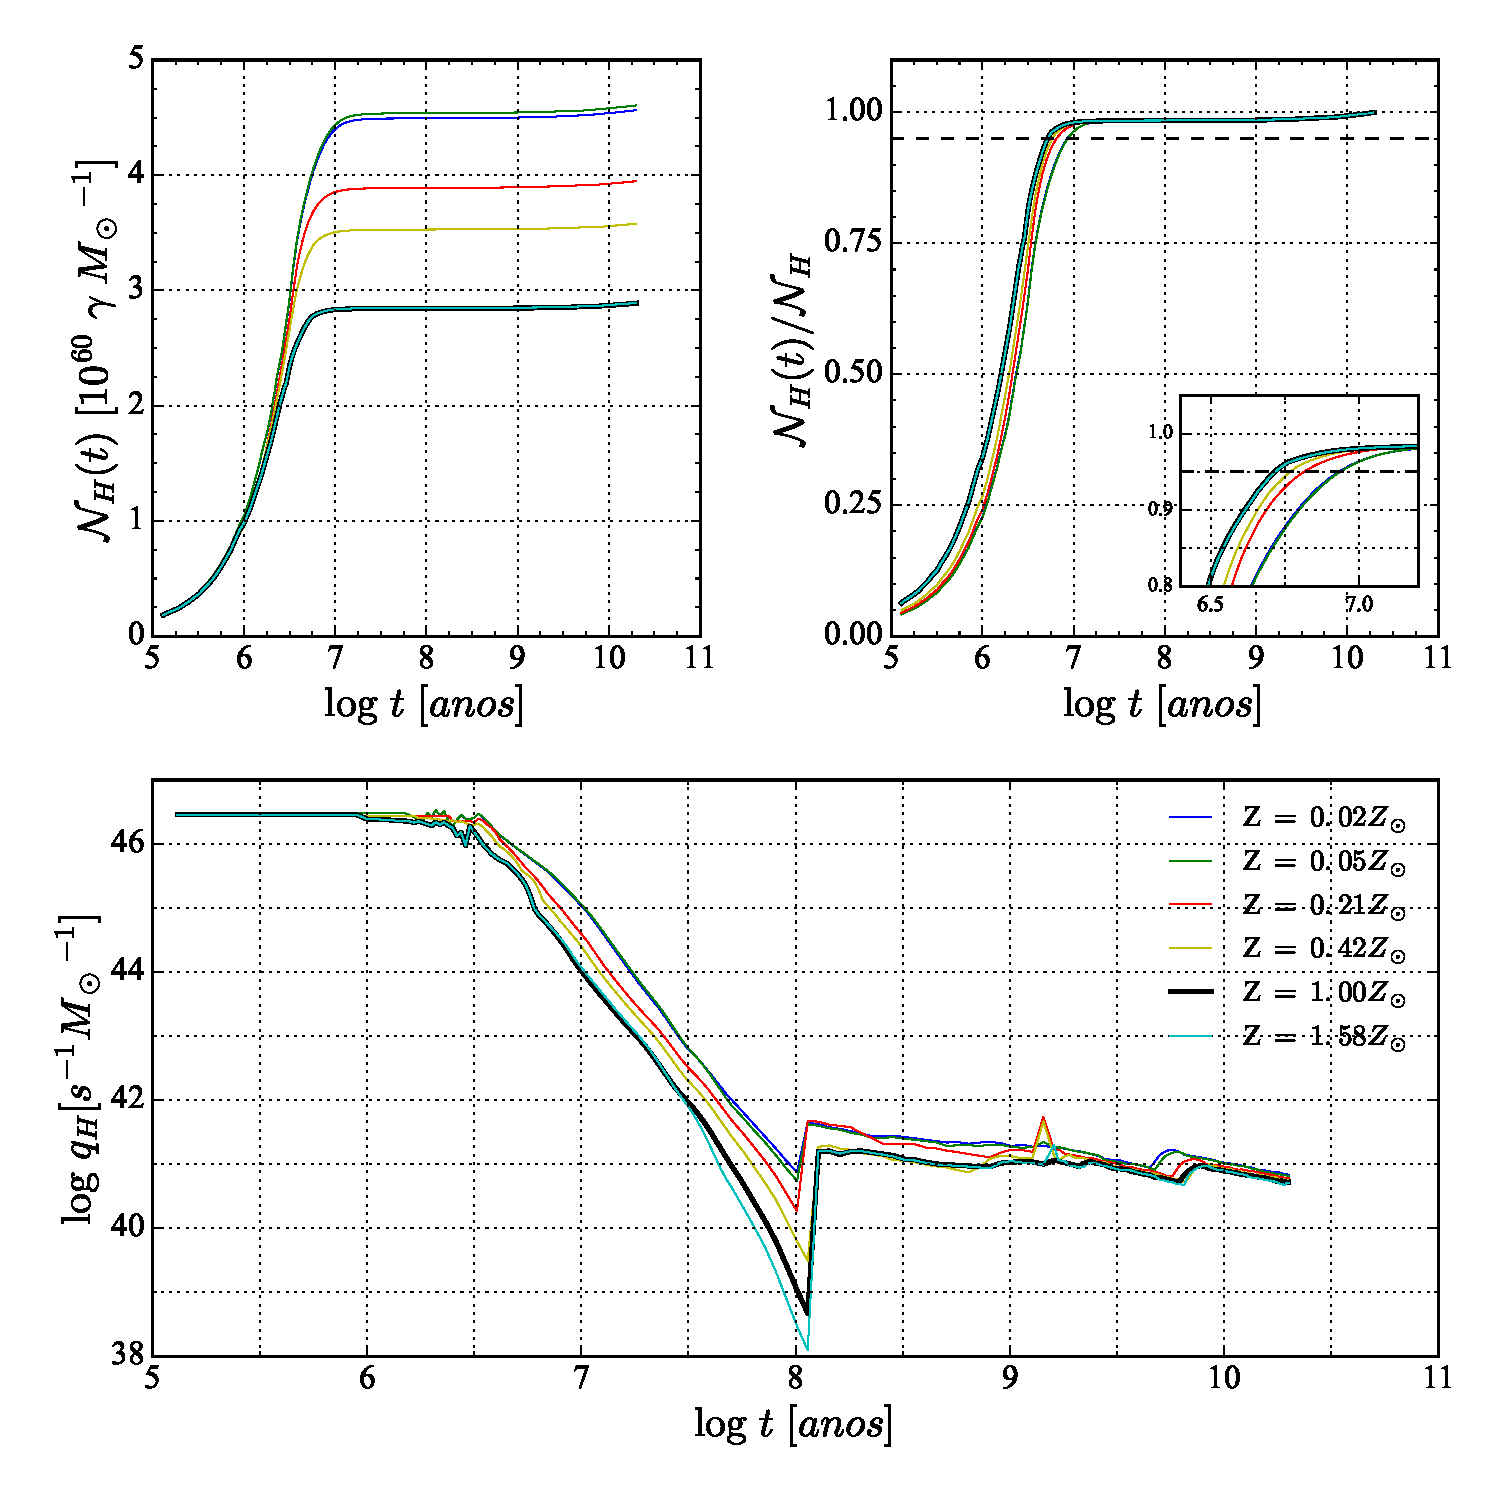
\includegraphics{Nh_logt_metBase_Padova2000_salp.pdf}}
	\resizebox{0.99\textwidth}{!}{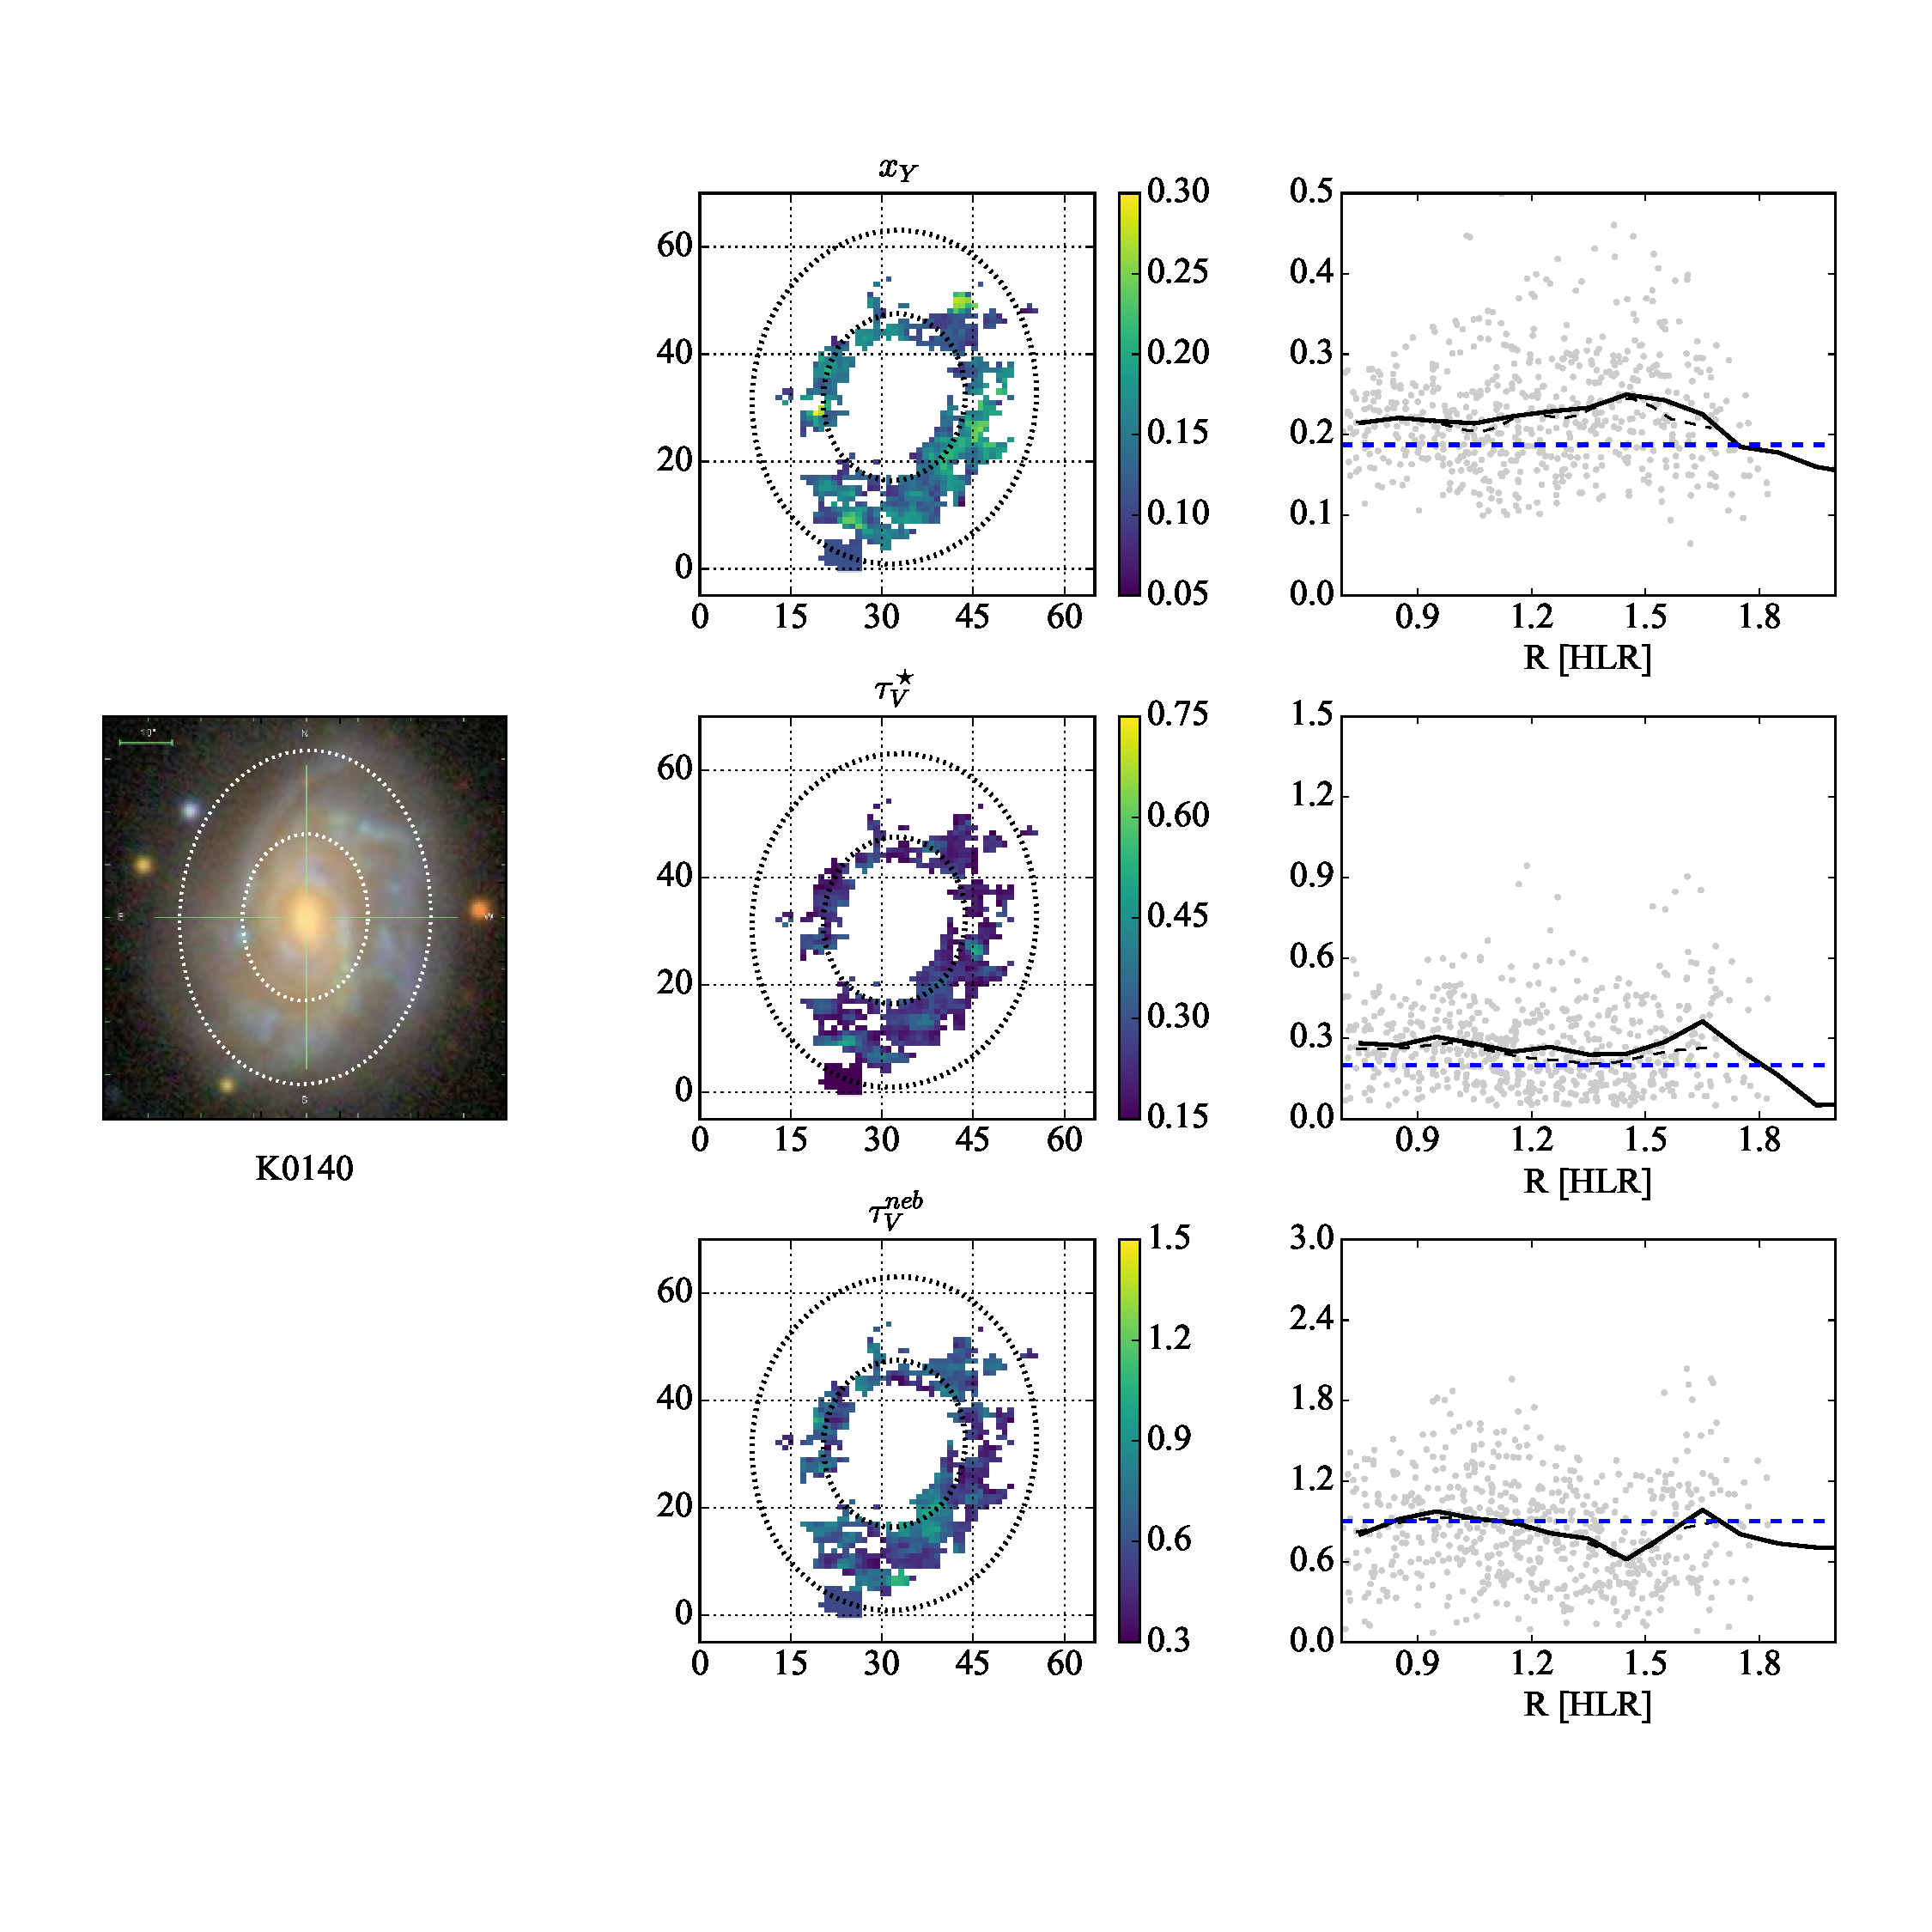
\includegraphics{figuras/K0140_xY_radialProfile_realsample.pdf}}
	\caption[Imagem e perfil radial de $x_Y$.]
	{\emph{Painel esquerdo}: Imagem da galáxia NGC1667 (CALIFA 140) do \SDSS. \emph{Painel central}:
	Mapa da fração percentual de luz proveniente das populações jovens ($x_Y$). \emph{Painel direito}:
	$x_Y$ contra a distância radial. Os pontos em cinza ao fundo são os valores para zonas. O perfil radial
	calculado em bins elipticos com espessura de 0.1 HLR é desenhado com uma linha preta contínua. Já
	linha tracejada representa o valor da mediana de $x_Y$ em bins de distância radial. Vemos que
	neste caso o valor do perfil radial de $x_Y$ acompanha o valor da mediana da distribuição dos
	valores para zonas. }
	\label{fig:K0140xYRadProf}
\end{figure}
 
% Figuras:
% - histograma tipos - histograma massa - influências dos cortes em tauV, raio e x_Y - Anexo: Lista
% de galáxias com massa, redshift, idade, etc ...

\section{Comparação entre as taxas de formação estelar}
\label{sec:synvsneb:SFR}

Com a síntese de populações estelares podemos calcular a história de formação estelar utilizando o
vetor cumulativo de massa ($\eta_\star(t_\star)$), que abarca a fração total de massa convertida em
estrelas para cada idade das populações da base ($\mu_j$). Então podemos calcular uma taxa de
formação dentro de um intervalo de tempo:
\begin{eqnarray}
	\eta_\star(t_\star)\ &=&\ \sum\limits_{t_{\star,j} < t_\star} \mu_j \\
	\overline{\mathrm{SFR}_\star}(t_\star)\ &=&\ M_\star \frac{(1\ -\ \eta_\star(t_\star))}{t_\star},
\end{eqnarray}
\noindent onde M${}_\star$ é a massa total convertida em estrelas durante toda a história de
formação estelar de uma galáxia. 

Como explicado em \ref{sec:emlines:SFR}, podemos medir a taxa de formação estelar recente medindo a
luminosidade intrínseca de \Halpha. Com as duas taxas de formação estelar, uma recente e uma em
função do tempo ($t_\star$) podemos encontrar o tempo que melhor correlaciona as duas medidas, de
forma a encontrar uma escala de tempo que defina as populações jovens ($t_{SF}$), ou seja,
populações recém formadas e que geralmente ainda residem nas regiões de formação estelar. Na Fig.
\ref{fig:SFRsynvsneb} vemos a correlação entre as SFRs, calculando
$\overline{\mathrm{SFR}_\star}(t_\star)$ para diferentes idades. Neste gráfico os cortes
definidos em \ref{sec:synvsneb:amostra} com relação a idade e coeficiente de extinção mínimos não
estão aplicados. O mesmo é válido para cortes em distância radial. Encontramos $t_{SF}$ como sendo
próximo a 32 milhões de anos. Esse número não está muito distante da escala de tempo de vida das
estrelas que produzem a maioria dos fótons capazes de produzirem a linha de \Halpha ($\sim10^7$
anos). Vemos também que o valor máximo de correlação não altera substancialmente entre $10^7$ e
$10^{7.5}$.

Este procedimento de comparação foi feito também em \citet{Asari.etal.2007a}, no qual os autores
encontraram $t_{SF}$ igual a 25 milhões de anos, para 82302 galáxias do \SDSS. A síntese de
populações estelares foi realizada utilizando o \starlight, mas com uma diferente IMF.

\begin{figure}
	\centering
	%\resizebox{0.99\textwidth}{!}{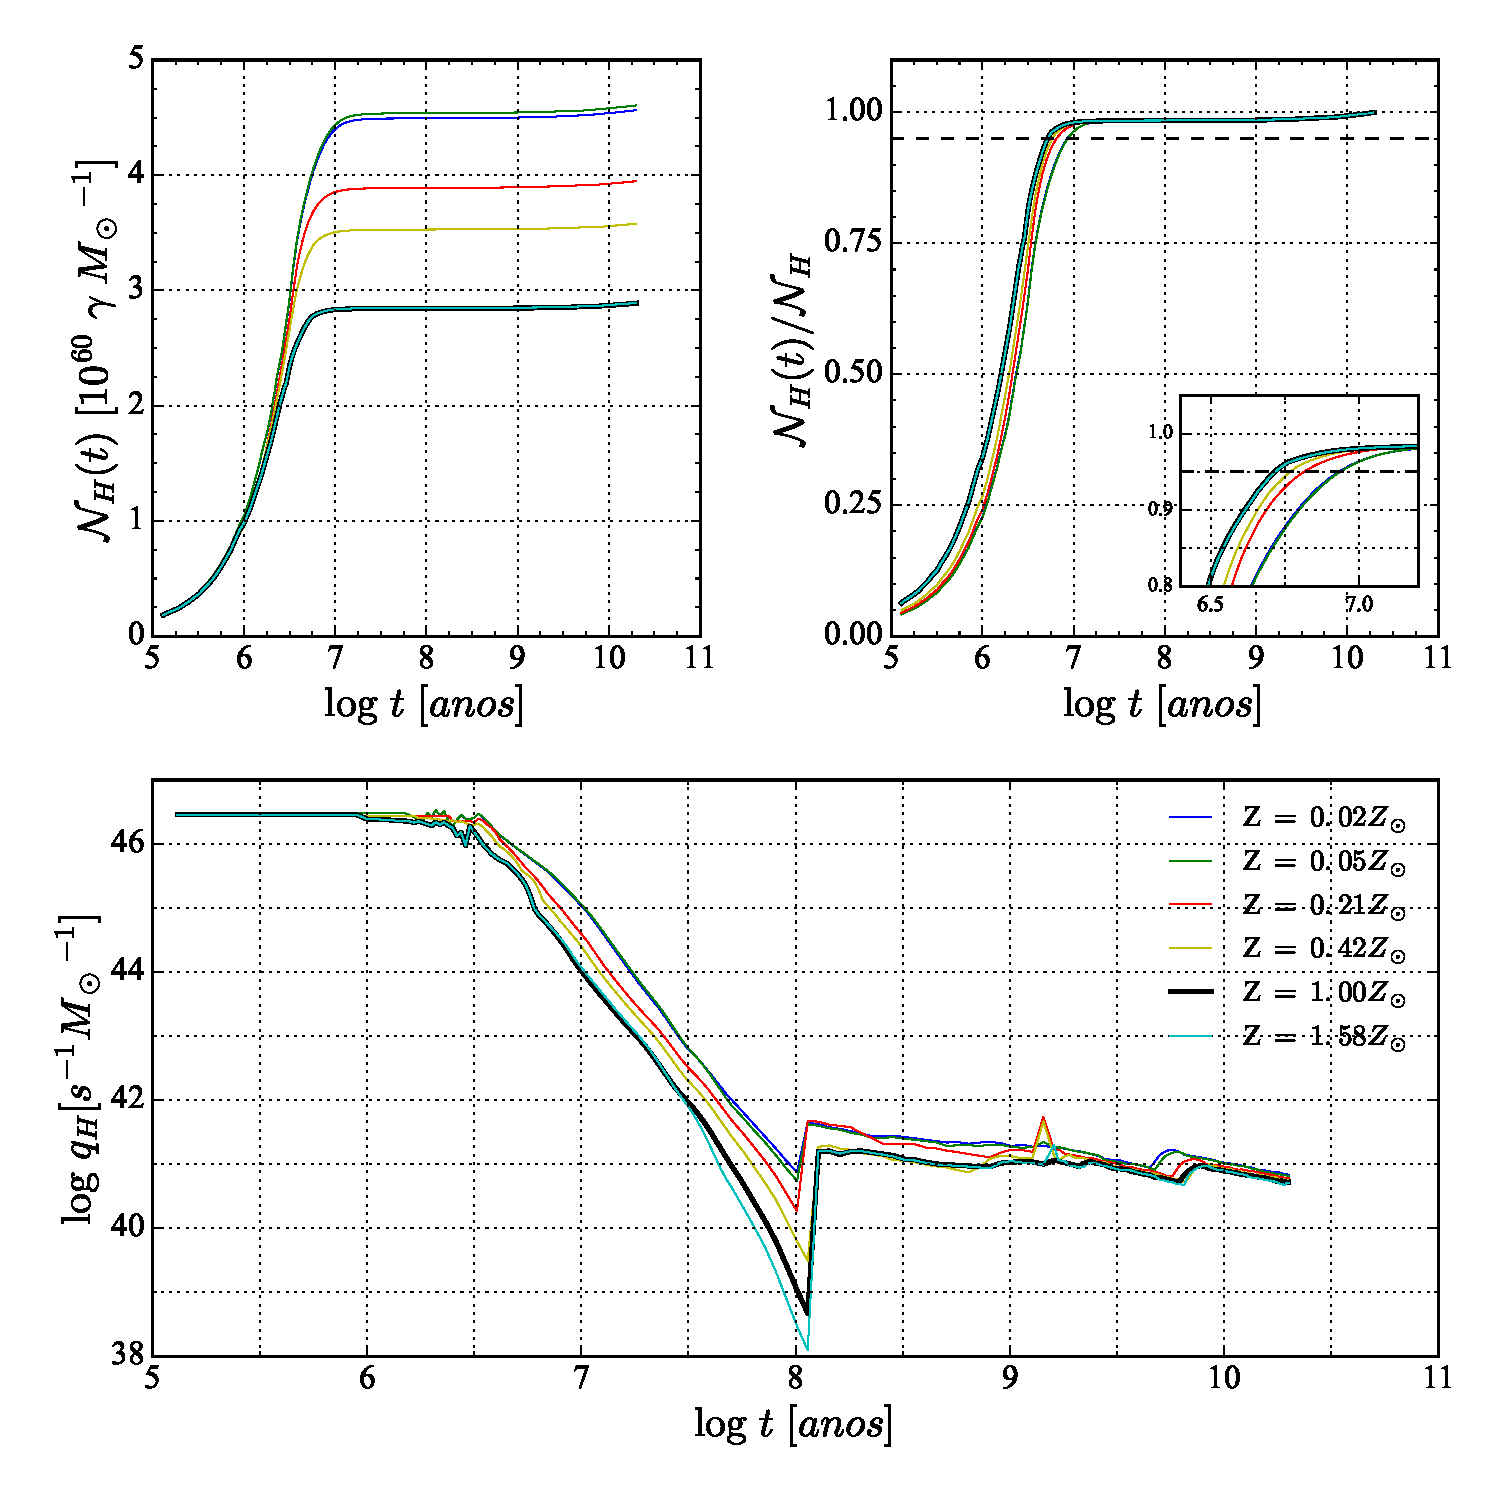
\includegraphics{Nh_logt_metBase_Padova2000_salp.pdf}}
	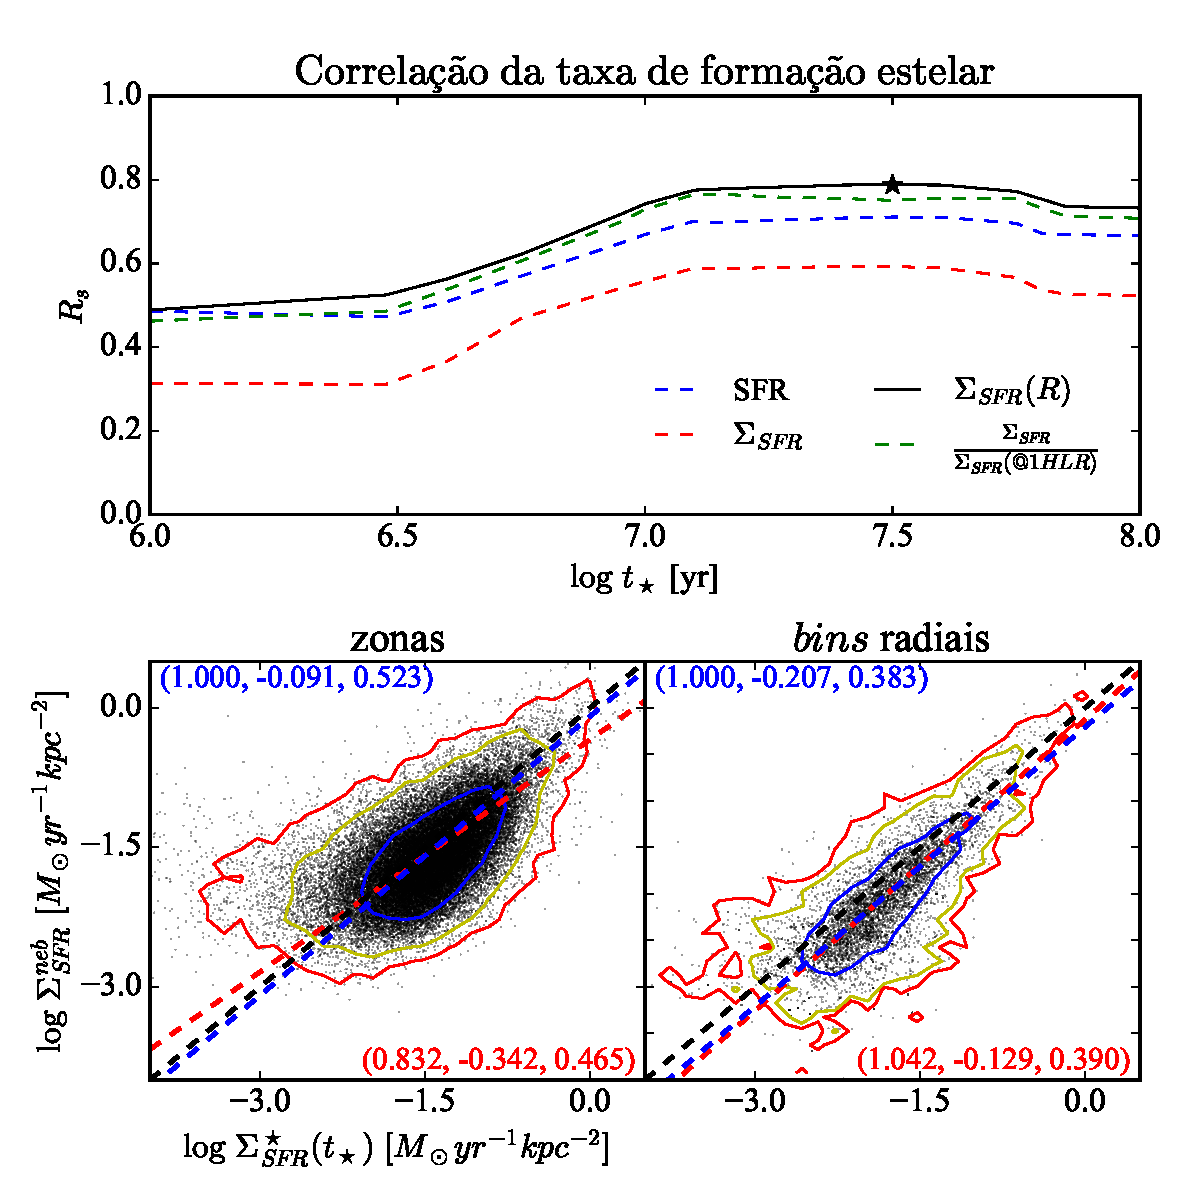
\includegraphics[scale=0.7, clip]{figuras/Rs_allSFR.pdf}
	\caption[Comparação entre as SFR.]
	{\emph{Painel superior}: O coeficiente de correlação de Spearmann entre as SFR para diferentes
$t_\star$. Para cada cor temos um tipo de cálculo de SFR e em linha preta contínua temos os valores
do coeficiente de Spearmann para os perfis radiais de $\Sigma_{\mathrm{SFR}}$, que possui o valor de
idade que utilizamos para ser nossa escala de tempo de formação estelar ($t_{SF})$. \emph{Demais
painéis}: Cada um dos gráficos de comparação entre as SFR utilizando $t_{SF}$. Essa idade foi a
escolhida pois é a que possui o melhor coeficiente de correlação entre os perfis radiais da
densidade de coluna da SFR $\Sigma_{\mathrm{SFR}}$. As correlações entre densidades de coluna são
mais confiáveis pois removem o termo $d^2$ existente no cálculo da SFR que induz uma correlação
direta entre $\mathrm{SFR}_\star$ e $\mathrm{SFR}_{\Halpha}$. Em cada painel a linha pontilhada
vermelha é o ajuste linear utlizando OLS bisector, em azul é o ajuste forçando que a inclinação
seja 1 e em preto é a bissetriz ($x = y$).}
	\label{fig:SFRsynvsneb}
\end{figure}
% Figuras:
% - melhor comparação e ajuste

\section{Comparação entre os coeficientes de extinção}
\label{sec:synvsneb:tauv}

A síntese de populações estelares realizadas pelo \starlight adota o mesmo modelo de extinção por
poeira explicado em \ref{sec:emline:datacube:tauvneb}, onde todas as populações são atenuadas pelo
mesmo fator $e^{-\tau_\lambda}$. Essa simplificação contraria tanto evidências observacionais quanto
estudos teóricos, que caminham para um cenário onde populações mais jovens são mais atenuadas pela
poeira que populações mais velhas. 

Apesar do modelo de extinção ser o mesmo, o coeficiente calculado por cada um dos procedimentos é
diferente, como podemos ver na Fig. \ref{fig:tauVsynvsneb}. Esta figura apresenta a comparação entre
os coeficientes de extinção para zonas e também para os perfis radiais. O coeficiente que vem do
\starlight é calculado no processo de ajuste espectral de maneira a evitar degenerescências nos
resultados, já o do decremento balmer representa melhor as regiões onde existem os observáveis
necessários para seu cálculo, ou seja, regiões onde existam linhas de \Halpha e \Hbeta, portanto,
regiões mais jovens. Verificamos que a medida que vamos sendo mais exigente com fração de luz
proveniente das populações jovens ($x_Y$), valor mínimo de $\tauVS$ e $\tauVN$, e distância radial
de cada zona considerada na comparação (ver Fig. \ref{fig:tauVsynvsnebMask}), as diferenças entre os
dois coeficientes diminui, iluminando um caminho que vamos nos aprofundar um pouco melhor no próximo
capítulo e que pode nos ajudar a um melhor entendimento do significado de $\tauVS$.

\begin{figure}
	\centering
	%\resizebox{0.99\textwidth}{!}{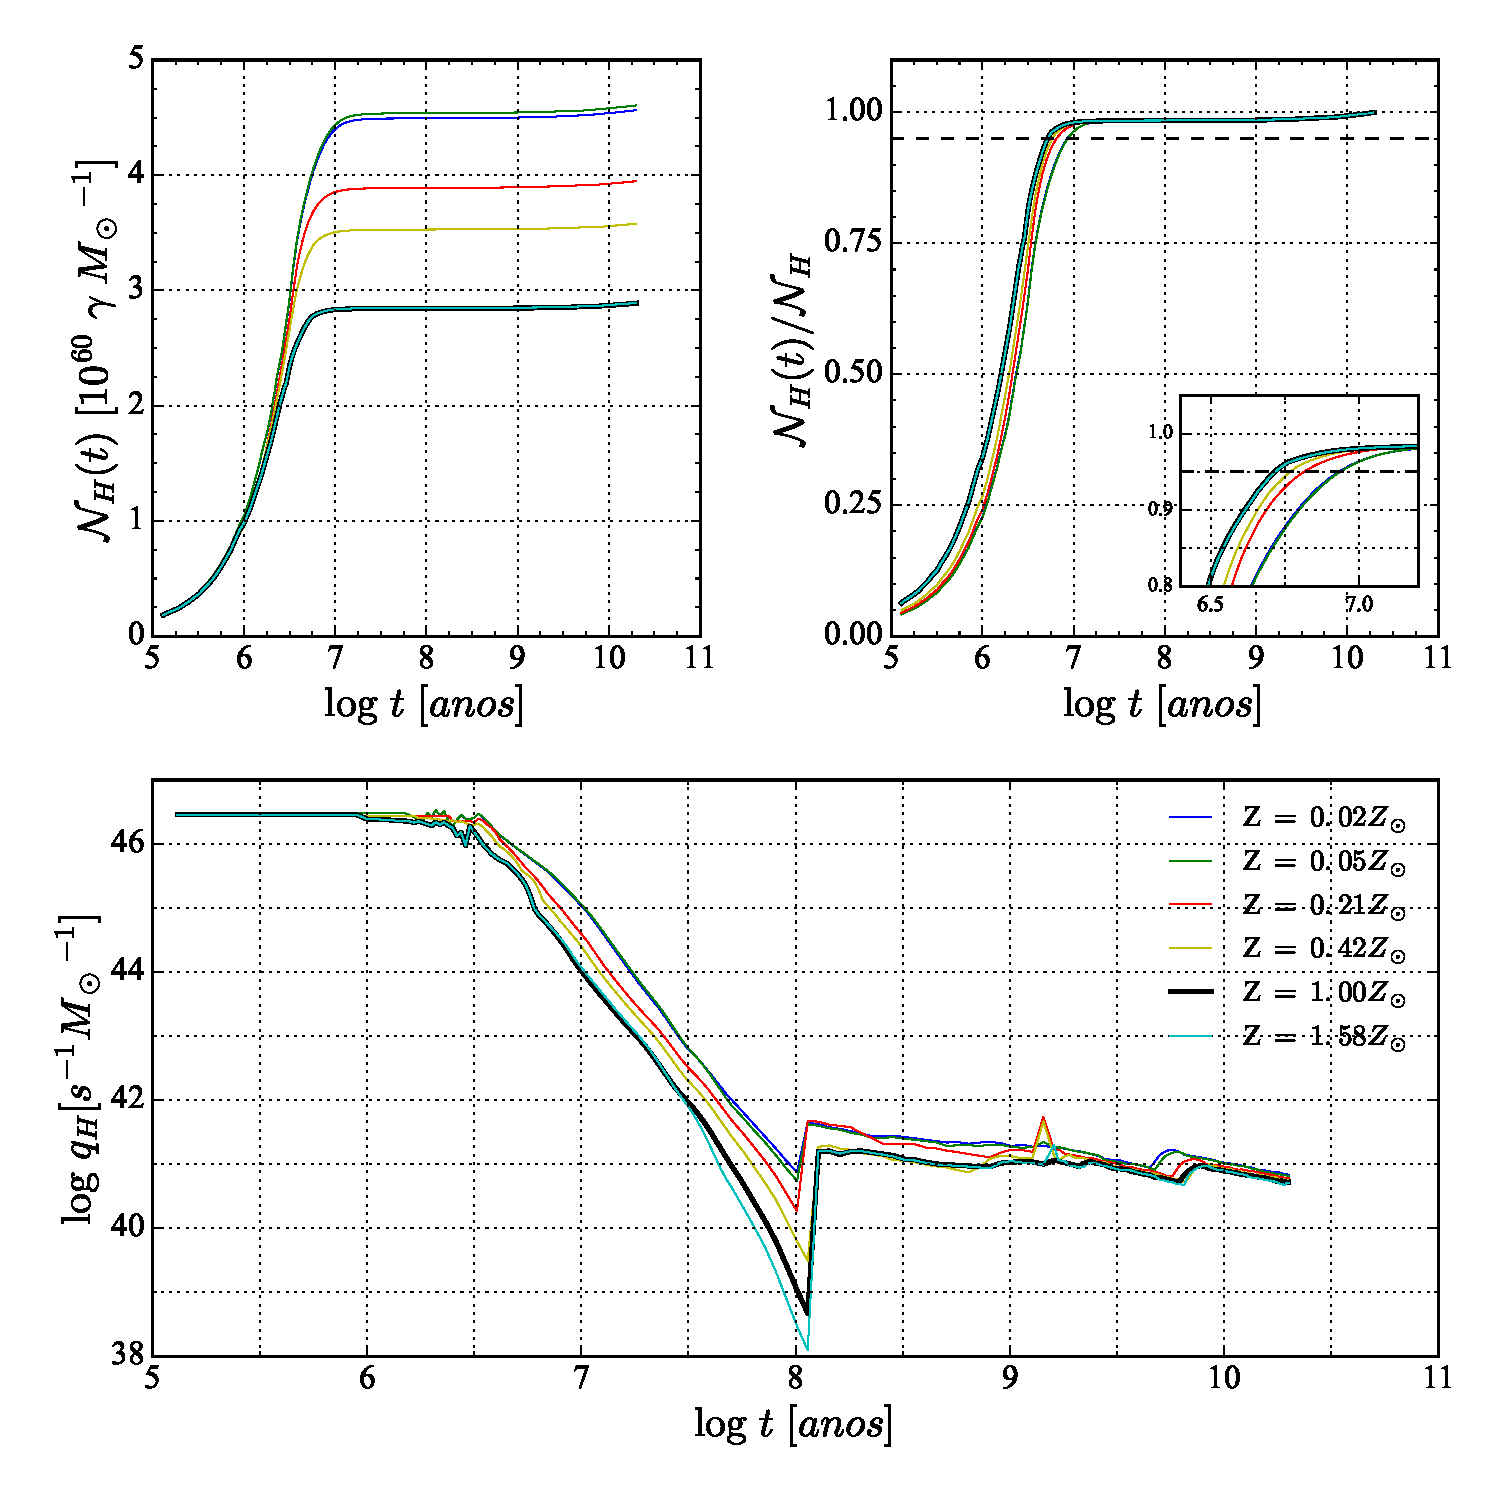
\includegraphics{Nh_logt_metBase_Padova2000_salp.pdf}}
	\resizebox{0.99\textwidth}{!}{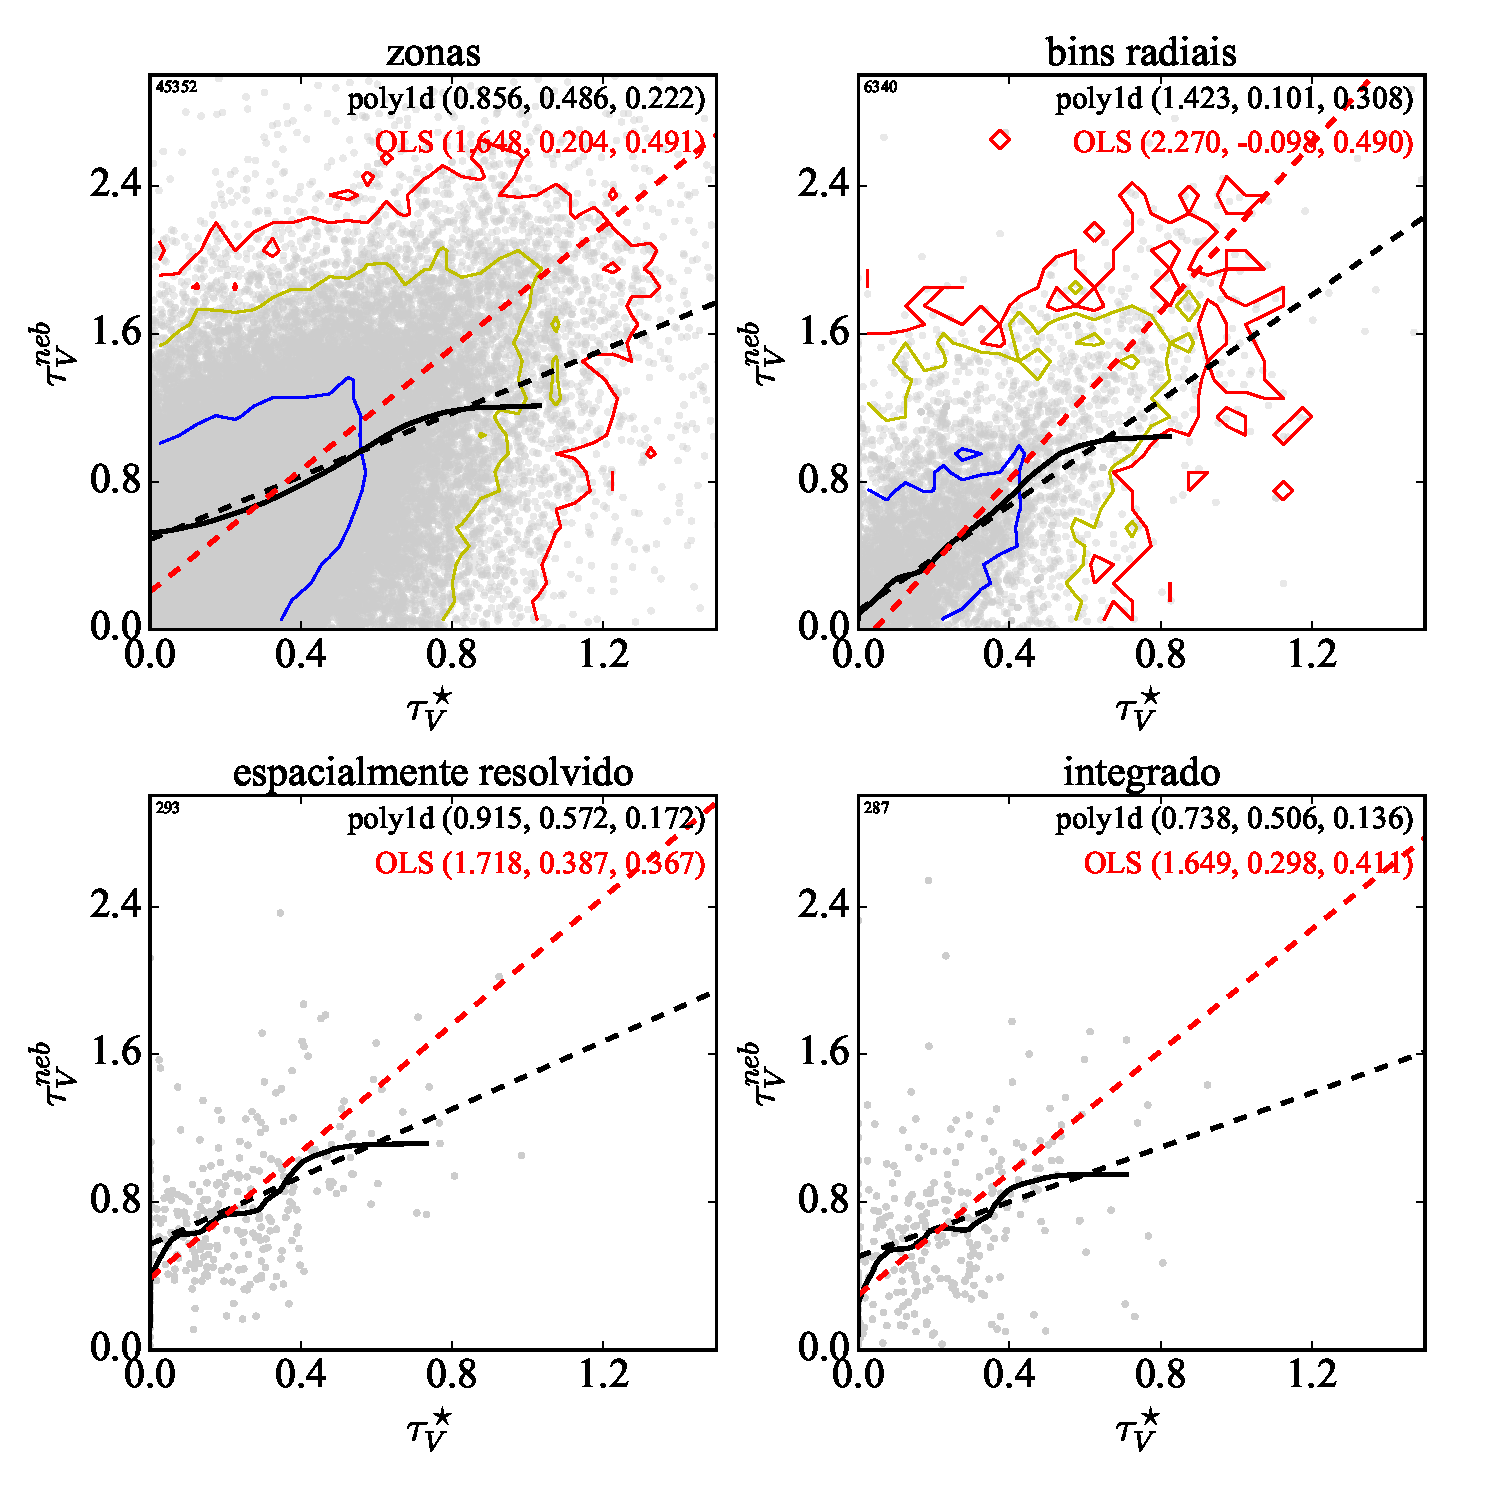
\includegraphics{figuras/CompareTauV.pdf}}
	\caption[Comparação entre os coeficientes de extinção.] 
	{Comparação entre os coeficientes de extinção por poeira provenientes da síntese ($\tauVS$) e
	do decremento de Balmer ($\tauVN$). Os contornos azul, amarelo e vermelho representam os intervalos
	de confiança ($1\sigma$, $2\sigma$ e $3\sigma$). A linha preta representa a mediana e as linhas
	pontilhadas representam o ajuste utilizando OLS bisector (vermelha) e mínimos quadrados (preta).
	Este gráfico não possui a máscara da definição da amostra aplicada. }
	\label{fig:tauVsynvsneb}
\end{figure}

\begin{figure}
	\centering
	%\resizebox{0.99\textwidth}{!}{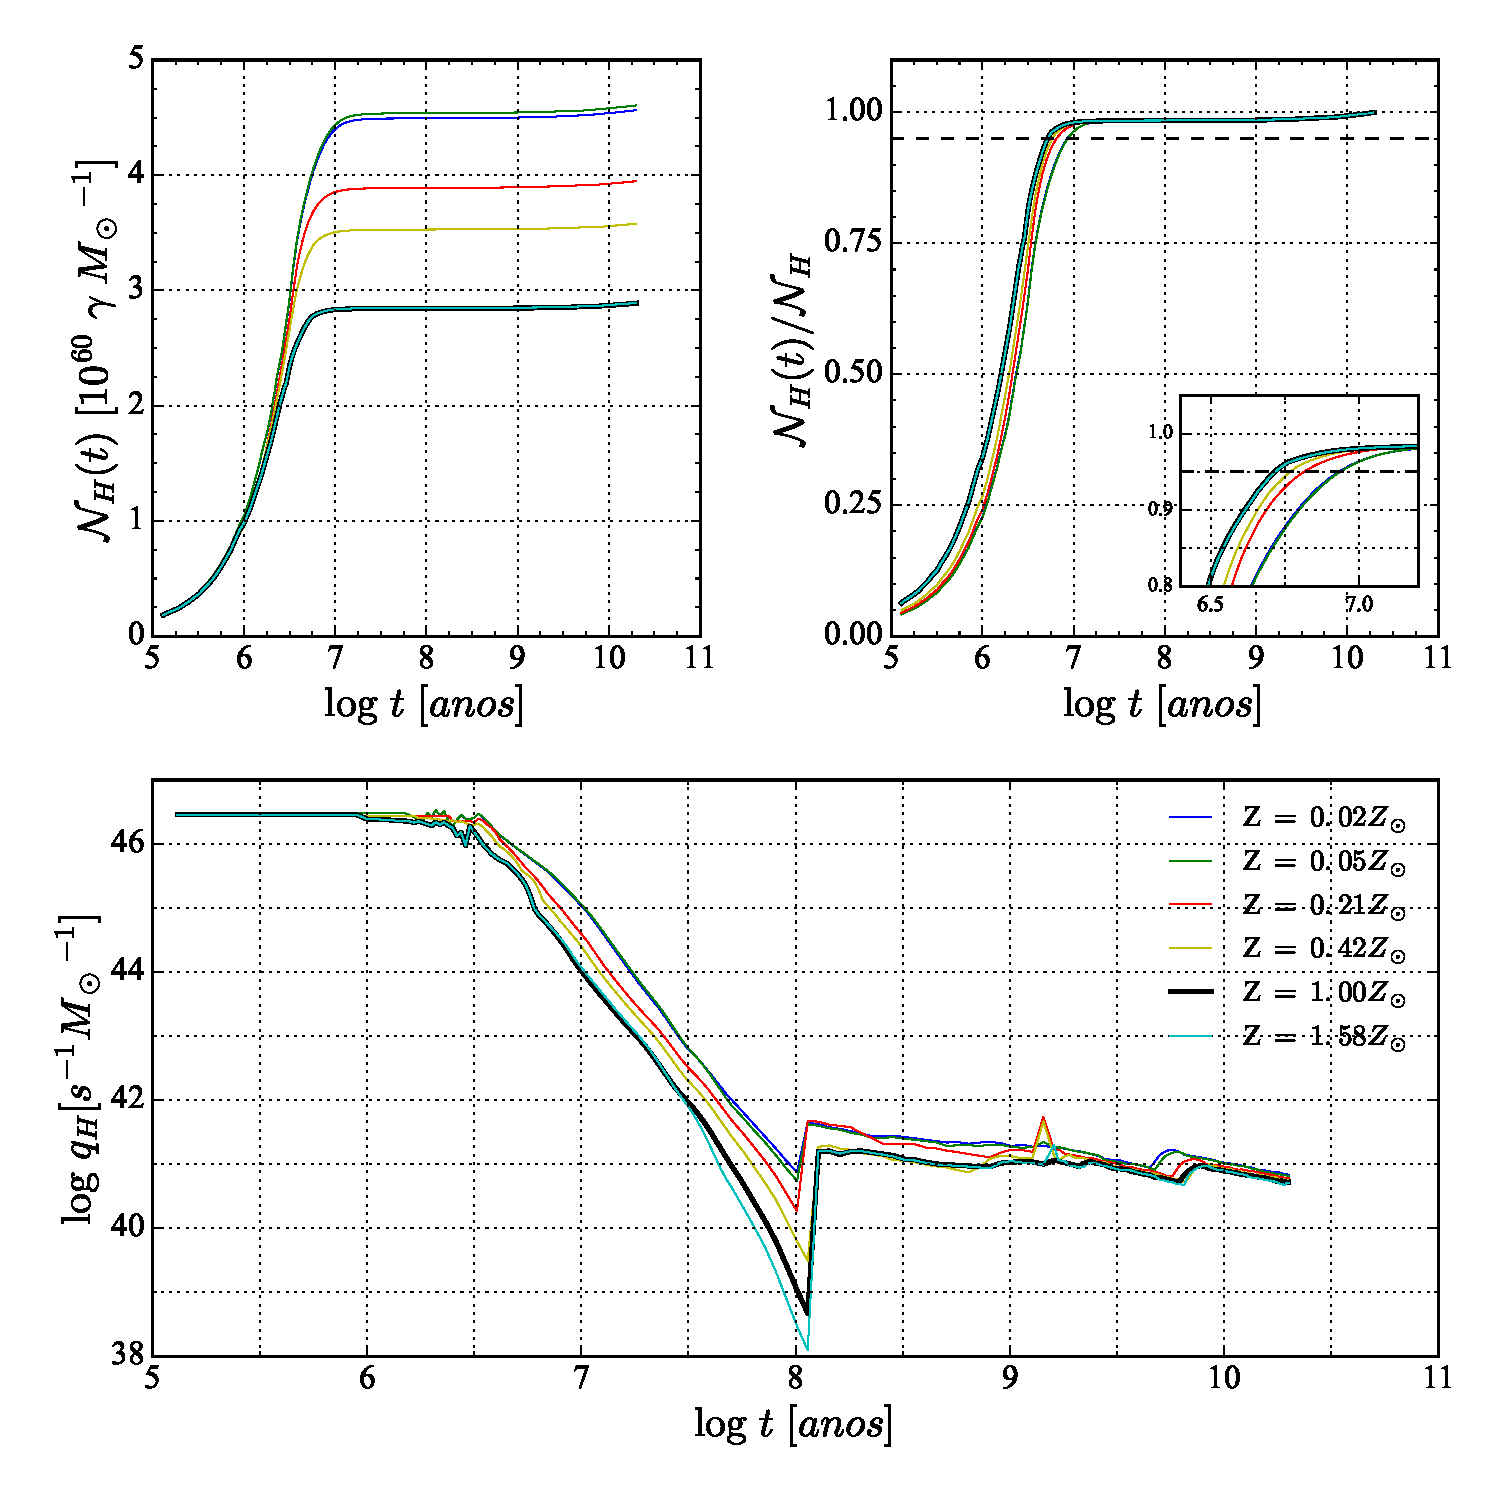
\includegraphics{Nh_logt_metBase_Padova2000_salp.pdf}}
	\resizebox{0.99\textwidth}{!}{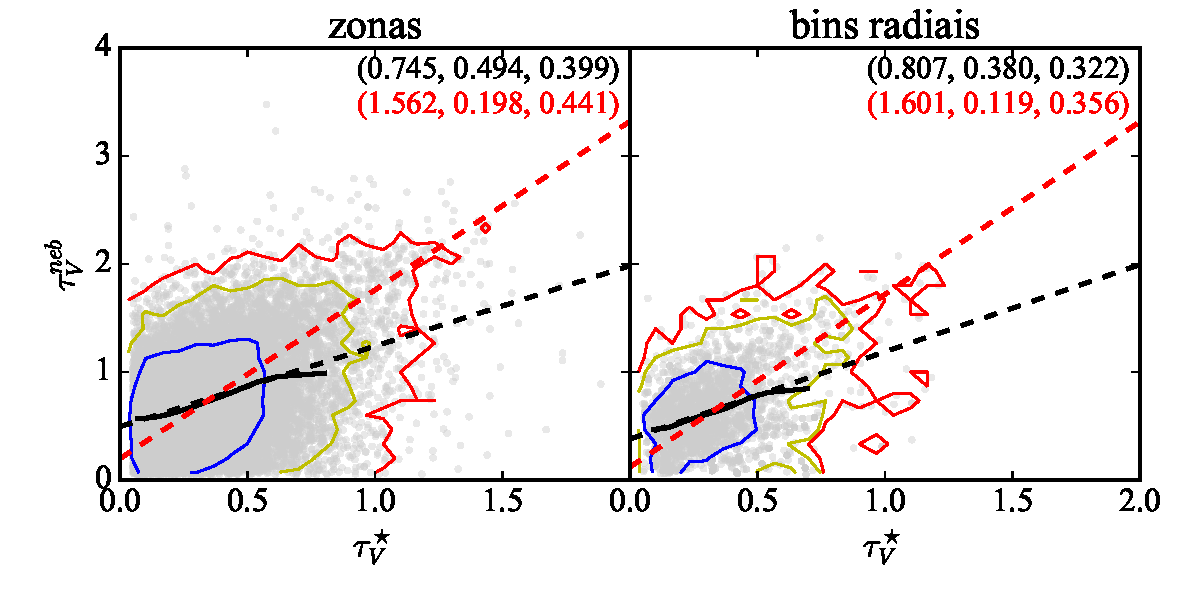
\includegraphics{figuras/CompareTauV_realsample.pdf}}
	\caption[Comparação entre os coeficientes de extinção (com máscara).]
	{Igual a Fig. \ref{fig:tauVsynvsneb} mas com a máscara de amostra aplicada.} 
	\label{fig:tauVsynvsnebMask}
\end{figure}

% Figuras:
% - Exemplo de diferenças entre mapas de tau_V
% - comparação entre tauV
% - x_Y

\section{Comparação entre as metalicidades}
\label{sec:synvsneb:Z}

No artigo de \citet{GonzalezDelgado.etal.2014b}, (GD14 daqui em diante) cuja versão completa está no
apêndice \ref{apendice:1} e eu tenho participação, analisamos a relação entre massa estelar
($M_\star$ - efeitos globais) e a densidade superficial de massa estelar ($\mu_\star$ - efeitos
locais) com a metalicidade estelar ($Z_\star$) de uma amostra de 300 galáxias do CALIFA de todos os
tipos morfológicos (desde E a Sd). \citet{Tremonti.etal.2004a} investigam a mesma relação, embora
para a metalicidade do gás ($\ZN$) e apenas para galáxias formadoras de estrelas\footnote{{\em
Star-forming galaxies}, com ativa formação estelar.}, essa relação é conhecida como relação
massa-metalicidade ({\em mass-metallicity relation} - MZR). Verificamos em nosso artigo que as
galáxias seguem uma boa MZR, mas expandindo um intervalo muito maior de metalicidade. A relação
totalmente estelar é mais inclinada que a relação comparando com a metalicdade do gás pois esta
última nos fornece informações sobre o estado atual do gás e a primeira, sobre toda a história de
formação estelar da galáxia. A metalicidade estelar para cada píxel (par $x,y$) é calculada segundo
a equação:
\begin{equation}
 	\label{eq:logZmass}
 	\langle \log Z_\star \rangle_{M,xy} = 
	\frac{ \sum_{tZ} M_{\star,tZ,xy} \times \log\ Z}{
	\sum_{tZ} M_{\star,tZ,xy} }.
\end{equation}

\citet{Sanchez.etal.2013a} analisa essa relação para $\sim 3000$ regiões \Hii mapeadas em 150
galáxias do CALIFA. Comparando nossos resultados com os obtidos por \citeauthor{Sanchez.etal.2013a}
(Fig. 2b em GD14) nestas regiões vemos que eles se distanciam conforme $M_\star$ diminui.
Após calculamos a metalicidade estelar considerando apenas populações jovens ($t_\star\ \leq$ 2
bilhões de anos) vemos que o resultado se aproxima melhor da tendência para as regiões \Hii.

Como citado em \ref{sec:emline:datacube:Zneb}, com a calibração de \citet{Marino.etal.2013a} temos
metalicidade nebular para aquelas regiões aonde temos medidas para todas as linhas envolvidas no
processo (\Hbeta, \oIII, \Halpha e \nII). Na Fig. \ref{fig:ZstarvsZneb} podemos ver a a relação
entre a densidade superficial de massa estelar e a metalicidade nos três painés de cima (zonas,
anéis elipticos e galáxias integradas) e, na mesma sequência, temos a comparação entre a
metalicidade nebular e estelar. Em cada gráfico aparecem as medianas para as metalicidades estelares
calculadas para diferentes intervalos de idades. A Figura nos mostra que para mesmos valores de
$\mu_\star$ a metalicidade estelar é mais alta para as estrelas mais jovens, o que parece ser um
resultado coerente imaginando que o meio onde as novas estrelas nascem vai enriquecendo, fazendo com
que novas estrelas tenham mais metalicidade. A metalicidade nebular parece ser muito menos sensível
às regiões mais massivas do que a metalicidade estelar. \citet{Zahid.etal.2014a}, analisando
galáxias com $z \lesssim 1.6$, argumentam que esse achatamento acontece quando o $M_\star \gg
M_{gas}$, assim a quantidade de oxigênio presa dentro das estrelas ({\em lock-up fraction}) de baixa
massa é da ordem daquela produzida pelas estrelas de alta massa. Os modelos de evolução química
evoluíram bastante nos últimos anos \citep[e.g., ][]{Lilly.etal.2013a, Peng.Maiolino.2014a,
Ascasibar.etal.2015a, Peng.Maiolino.Cochrane.2015a} e esperamos que logo tenhamos melhores
resultados na área. O tema é muito interessante e tem muito ainda a ser explorado, principalmente os
efeitos locais, quando analisamos esta relação internamente nas galáxias e seus efeitos em
parâmetros globais.

\begin{figure}
	\centering
	%\resizebox{0.99\textwidth}{!}{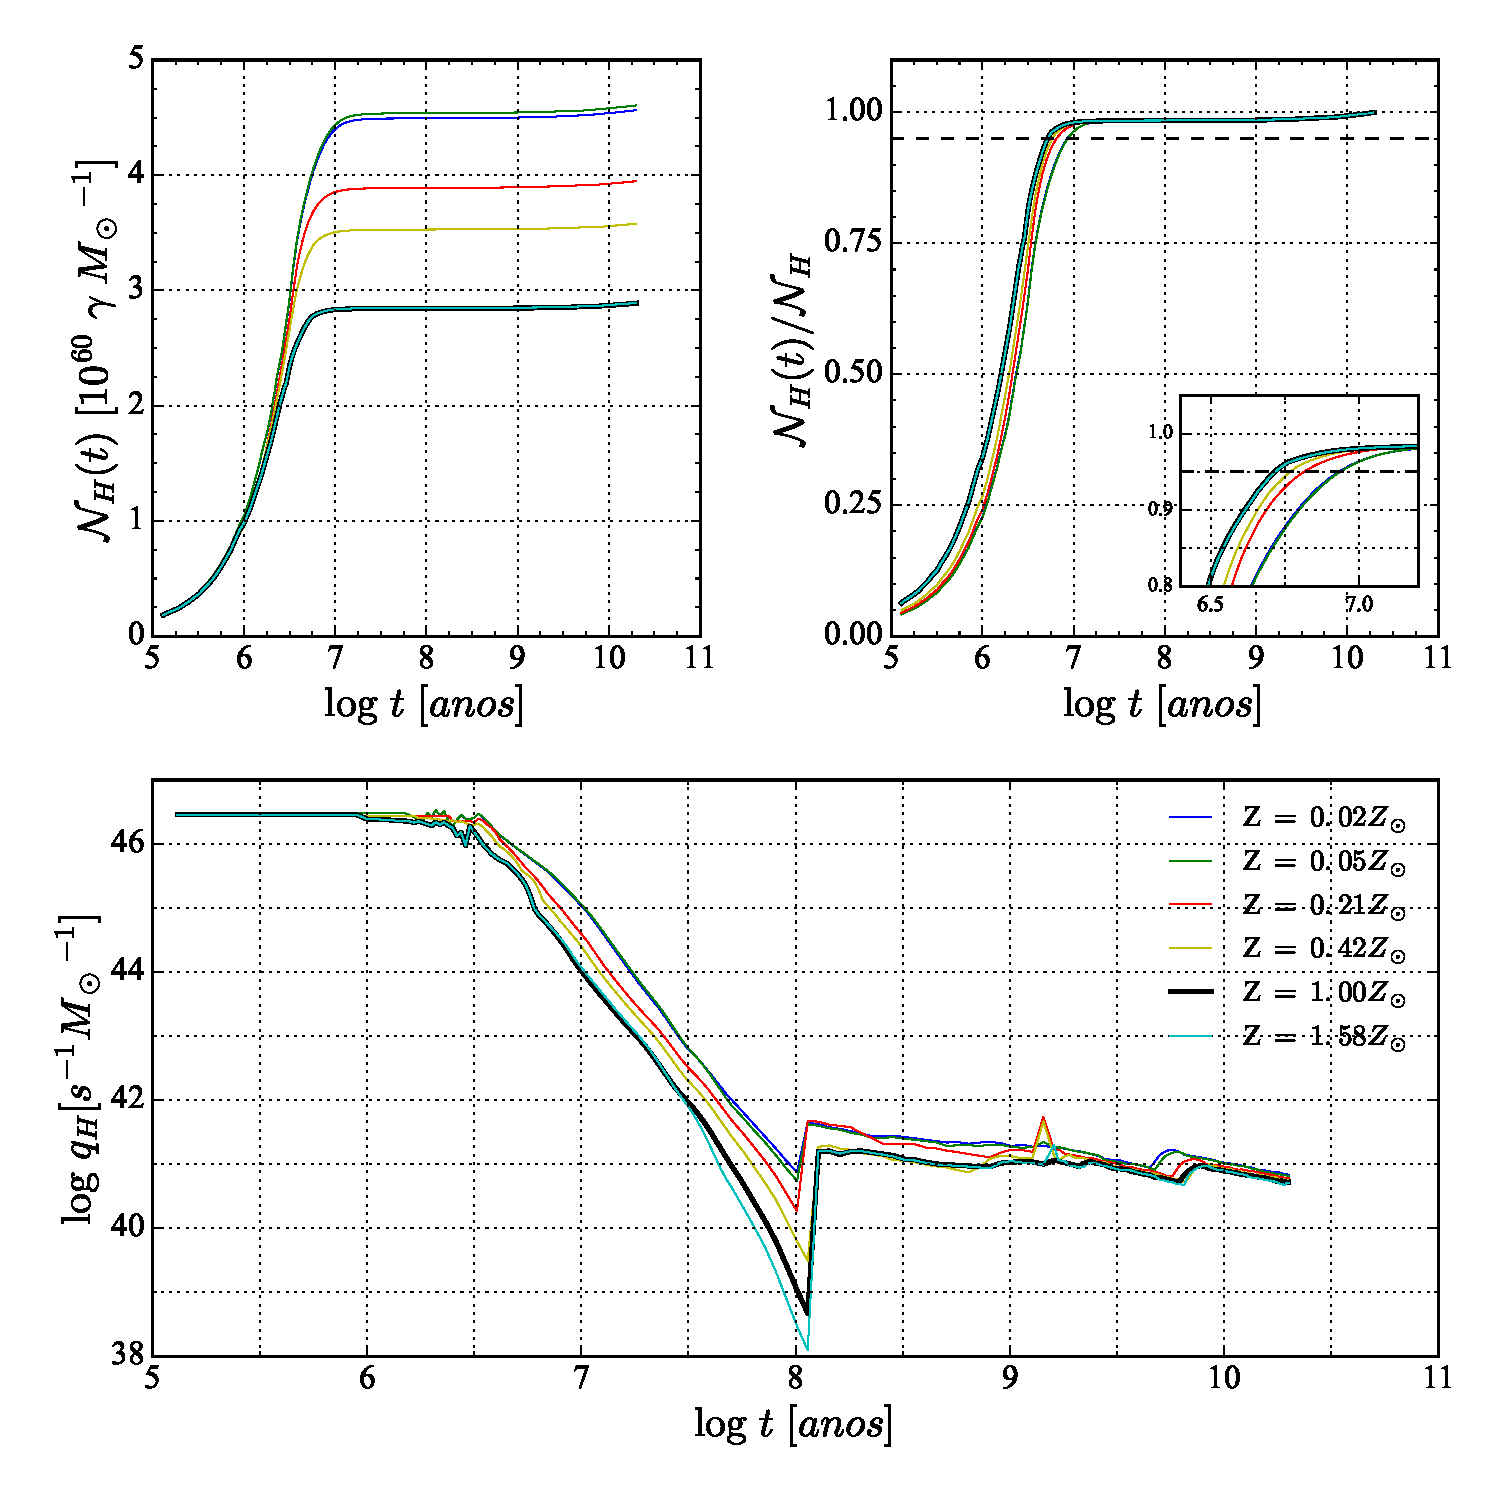
\includegraphics{Nh_logt_metBase_Padova2000_salp.pdf}}
	\resizebox{0.99\textwidth}{!}{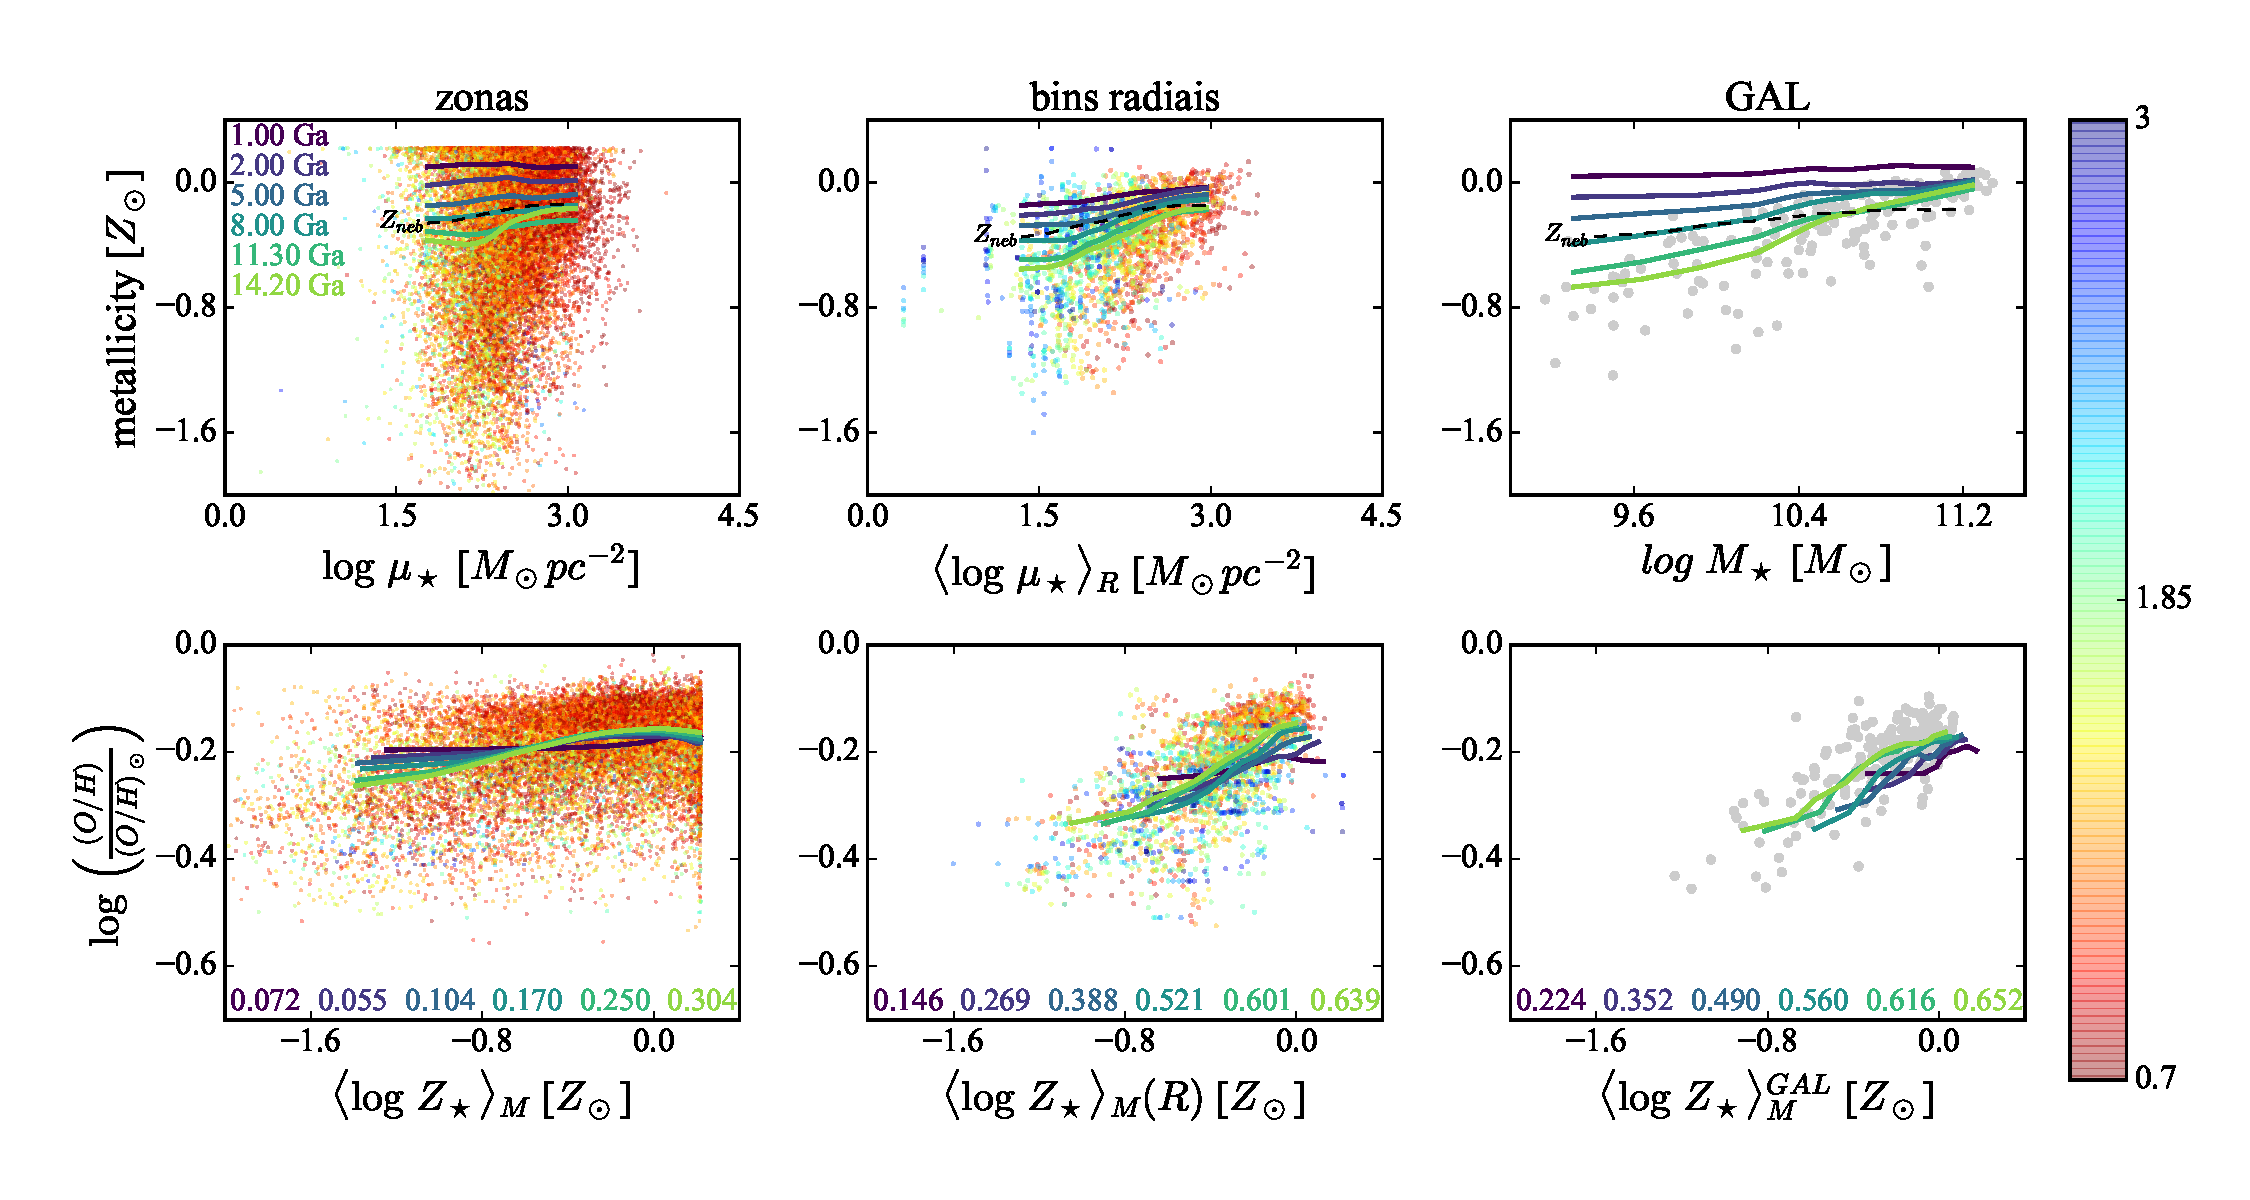
\includegraphics{figuras/stellar_muZR_realsample.pdf}}
	\caption[Relação $\mu$ZR e comparação entre as metalicidades.]
	{\emph{Painéis superiores}: relação $\mu$ZR para zonas (painel esquerdo), {\em bins} radiais
(painel central) e galáxias integradas (painel direito). Os pontos desenhados em cada gráfico
representam $\meanM{\log Z_\star}$ calculado para todas as populações com distintas idades,
coloridos pela distância radial (barra de cores em HLR). Cada gráfico possui a mediana da
distribuição de $\meanM{\log Z_\star}$ para diferentes intervalos de população ($t_\star \leq$ 1,
2, 5, 8, 11.3 e 14.2 bilhões de anos), além da mediana para $\ZN$
($\log\left((O/H)/(O/H)_\odot\right)$). \emph{Painéis inferiores}: Comparação $\meanM{\log Z_\star}$
e $\ZN$ seguindo a mesma configuração acima (zonas, raio e integrado) com as medianas por diferentes
intervalos de população no cálculo de $\meanM{\log Z_\star}$ também. Seguindo o mesmo padrão de
cores para as medianas, abaixo de cada gráfico vemos o coeficiente de correlação de Spearmann entre
$\meanM{\log Z_\star}$ e $\ZN$.}
	\label{fig:ZstarvsZneb}
\end{figure}

%Estudos recentes apontam valores similares para o tempo de depleção do gás \citep[e.g., ][ver tabela 5 e
%referências.]{Leroy.etal.2013a}. As galáxias mais massivas completaram seu enriquecimento químico a
%muitas eras atrás, com a história de formação estelar geralmente aproximanda a um único largo broto
%de formação estelar. Hoje, as galáxias menos massivas são aquelas que possuem maior atividade de
%formação estelar. Esse fenômeno é conhecido como {\em Downsizing} \myojo{blue}{REFS?}.

% Quando calculamos a metalicidade média das populações jovens das galáxias, estamos olhando para as
% populações estelares de galáxias menos massivas, mais jovens e com atividade de formação estelar
% intensa, portanto com um interva

% Figuras:
% - comparação entre metalicidades

%% End of this chapter
